\documentclass[addpoints, answers]{exam} % добавить или удалить answers в скобках, чтобы показать ответы
%\usepackage[utf8]{inputenc}
%\usepackage[russian]{babel}
%\usepackage[OT1]{fontenc}
%\usepackage{booktabs}
%\usepackage{amsmath}
%\usepackage{tikz}
%\usepackage{amsfonts}
%\usepackage{amssymb}
%\usepackage[left=2cm,right=2cm,top=2cm,bottom=2cm]{geometry}
%\DeclareMathOperator{\E}{\mathbb{E}}
%\DeclareMathOperator{\Var}{\mathbb{V}\mathrm{ar}}
%\DeclareMathOperator{\Cov}{\mathbb{C}\mathrm{ov}}
%\let\P\relax
%\DeclareMathOperator{\P}{\mathbb{P}}
\newcommand{\cN}{\mathcal{N}}
\newcommand{\hbeta}{\hat{\beta}}

\usepackage{floatrow}
%\newfloatcommand{capbtabbox}{table}[][\FBwidth]

\input{title_bor_utf8}

\title{Подборка вступительных экзаменов в магистратуру. \\Факультет экономики, НИУ-ВШЭ}
\author{Коллектив авторов}


\begin{document}

\pagestyle{headandfoot}
\runningheadrule
\firstpageheader{НИУ-ВШЭ}{Подборка вступительных экзаменгов в магистратуру} {стр. \thepage\ из \numpages}
\firstpageheadrule
\runningheader{НИУ-ВШЭ}{Подборка вступительных экзаменгов в магистратуру} {стр. \thepage\ из \numpages}
\firstpagefooter{}{}{}
\runningfooter{}{}{}
\runningfootrule


\maketitle
\tableofcontents
\newpage

\hqword{Задача}
\hpgword{Страница}
\hpword{Максимум}
\hsword{Баллы}
\htword{Итого}
\pointname{\%}
%\renewcommand{\solutiontitle}{\noindent\textbf{Решение:}\par\noindent}
\renewcommand{\solutiontitle}{}

%Таблица с результатами заполняется проверяющим %работу. Пожалуйста, не делайте в ней пометок.

%\begin{center}
 % \gradetable[h][questions]
%\end{center}

\section{2007}

\subsection{Вариант A}
\begin{questions}

\question Найдите 
\[
\lim_{x \to 2}\frac{\sqrt[3]{6+x}-\sqrt{x+2}}{\sqrt[3]{25+x}-\sqrt{7+x}}
\]
\question Матрица вида А=
$\left( \begin{array}{cc}
a & b\\
c & -a
\end{array} \right)$ 
имеет собственное значение $\lambda_1=3$, которому соответствует собственный вектор 
$\left( \begin{array}{c}
1\\
1
\end{array} \right).$ Второй собственный вектор этой матрицы --- 
$\left( \begin{array}{c}
1\\
-2
\end{array} \right).$ 
Вычислите определитель данной матрицы.\\
\question Найдите стационарные точки функции $f(x,y)=e^{2x+3y}(8x^2-6xy+3y^2)$ и определите их тип.\\
\question Найдите минимумы и максимумы функции $f(x,y)=2x^2-3xy-2y^2$ при ограничении $x^2+y^2=10$.\\
\question Найдите решение дифференциального уравнения $xy'-6y=10x^4-16x^2$, удовлетворяющее условию $y(1)=0$. Постройте эскиз графика данного решения. \\
\question Найдите общее решение дифференциального уравнения $y''-4y'+3y=e^{2x}$.\\
\question Время, проводимое покупателем в супермаркете, можно считать нормально распределенной случайной величиной. Известно, что математическое ожидание этой случайной величины составляет 1 час 20 минут, а стандартное отклонение равно 15 минутам. Найдите при этих условиях вероятность того, что из трех незнакомых между собой покупателей хотя бы один проведет в супермаркете более полутора часов.\\
\question Функция плотности двумерной случайной величины $(X,Y)$ имеет вид\\
$p(x,y)=\begin{cases}
c(-x),\text{ если } x\in [0;1],y \in [1;2]\\
0,\text{ иначе }
\end{cases}$\\

Найдите:
\begin{parts}
\part значение константы с
\part вероятность того, что $Y\leq2X$
\part математическое ожидание $\E(Y)$
\end{parts}
\question Проверка 175 старых домов города показала, что в 56 из них электропровода требуют срочного ремонта. На уровне значимости 5\% проверьте гипотезу о том, что доля всех старых домов города, в которых требуется срочный ремонт электропроводки, составляет не менее 33\%.\\
\item По данным 22 наблюдений в рамках классической нормальной линейной регрессии была получена модель $\hat{Y}_i=\hat{\alpha}+\hat{\beta}X_i$ с коэффициентом детерминации $R^2=0.93$. Проверьте гипотезу об адекватности этой регресии
\end{questions}


\subsection{Вариант A1}
\begin{questions}
\question Найдите 
\[
\lim_{x\to 0}\frac{\sqrt{1+\tg x}-\sqrt{1-\tg x}}{\sin x}
\]
\question Матрица вида А=
$\left( \begin{array}{cc}
0.6 & 0.8\\
c & d
\end{array} \right)$ 
коммутирует с матрицей B=
$\left( \begin{array}{cc}
0 & 1\\
-1 & 0
\end{array} \right)$, то есть выполняется равенство $A\cdot B=B\cdot A$. Найдите константы $c,d$ и матрицу $A^{-2}$ (матрицу, обратную матрице $A^2=A\cdot A$).\\

\question Найдите стационарные точки функции $f(x,y)=x^3+y^3+21x^2+18xy+21y^2$ и определите их тип.\\
\question Найдите минимумы и максимумы функции $f(x,y)=x^3\cdot y^4$ в области $x>0,y>0$ при ограничении $3x+4y=7$.\\
\question Найдите решение дифференциального уравнения $xy'+3y=x^2$, удовлетворяющее условию $y(1)=1/3$. Постройте эскиз графика найденного решения. \\
\question Найдите общее решение дифференциального уравнения $y''-y=e^{2x}$.\\
\question Синоптики Аляски и Чукотки независимо друг от друга предсказывают погоду (<<ясно>> или <<пасмурно>>) в Беринговом проливе, ошибаясь с вероятностями 0.1 и 0.2 соответственно. Их предсказания на завтра разошлись. Какова вероятность того, синоптики Аляски ошиблись?\\
\question Функция плотности двумерной случайной величины $(X,Y)$ имеет вид\\
$p(x,y)=\begin{cases}
c,\text{ при } x\in [0;1],y \in [0;1], y\geq x\\
0,\text{ в остальных случаях }
\end{cases}$\\
Найдите:
\begin{parts}
\part значение константы с
\part вероятность того, что $Y\leq 2X$
\part математическое ожидание $\E(Y)$
\end{parts}
\question Медицинское обследование 180 пациентов показало, что у 63 из них наблюдалось улучшение состояния после лечения новым препаратом. Найдите 95\% доверительный интервал для теоретической доли тех пациентов, у которых може наблюдаться такое улучшение.\\
\question По данным 30 наблюдений в рамках классической нормальной линейной регрессии была получена модель $\hat{Y}_i=\hat{\alpha}+\hat{\beta}X_i$, причём $\hat{\beta}=2.04, \hat{\sigma}_{\hat{\beta}}=0.75$. Проверьте адекватность этой регрессии.
\end{questions}

\subsection{Вариант В}
\begin{questions}
\question Найдите предел
\[
\lim_{x\to 0} \frac{\sin 3x-\tg 4x}{\arcsin 2x}
\]
\question Найдите матрицу $X$ из уравнения $A\cdot X\cdot A'=B$, где $A=\left(\begin{array}{cc}
2 & 7\\
1 & 4
\end{array}\right), B=\left(\begin{array}{cc}
7 & 2\\
2 & 0
\end{array}\right), A'=\left(\begin{array}{cc}
2 & 1\\
7 & 4
\end{array}\right)$ --- матрица, транспонированная по отношению к матрице А.\\
\question Найдите минимумы и максимумы функции $f(x,y)=\ln x+\ln y-3x-y-6xy$.\\
\question Найдите решение дифференциального уравнения $y''+y'-2y=3$, удовлетворяющее условиям $y(0)=0$, $y'(0)=0$. Постройте эскиз графика найденного решения.\\
\question Время обслуживания одного вызова на междугородней телефонной станции можно считать нормально распределенной случайной величиной. При этом математическое ожидание составляет 1,5 минуты, а стандартное отклонение равно 0,5 минуты. Найдите при этих условиях вероятность того, что время обслуживания хотя бы одного из двух независимых вызовов составит более двух минут.\\
\question Функция плотности случайной величины $X$ имеет вид\\
$f(x,y)=\begin{cases}
c(1-|x|), |x|\leq 1\\
0, |x|>1.
\end{cases}$\\
Найдите значение константы $c$, математическое ожидание и дисперсию величины $X$.\\
\question Для случайной выборки, состоящей из 8 наблюдений, извлеченных из нормальной генеральной совокупности, был получен следующий 90\% доверительный интервал для математического ожидания $\mu$: $18,1<\mu< 18.9$. Постройте 95\% доверительный интервал для этого математического ожидания.\\
\question По данным 26 наблюдений в рамках классической нормальной регрессии была получена модель $\hat{Y}_i=\hat{\alpha}+\hat{\beta}X_i$, в которой $\hat{\beta}=2.0598$, $\hat{\sigma}_{\hat{\beta}}=0.0153$. На уровне значимости 5\% проверьте гипотезу
$\begin{aligned}
H_0&: \beta=2\\
H_a&: \beta\ne 2
\end{aligned}$
\end{questions}

\subsection{Вариант В1}
\begin{questions}
\question  Найдите предел
\[
\lim_{x\to 0} \frac{\sqrt{1+x+x^2}-1}{x}
\]
\question Матрица $A=\left(\begin{array}{cc}
4 & a \\ 
-6 & -a
\end{array}\right)$ имеет собственное значение $\lambda=1$. Найдите константу $a$ и собственные значение матрицы $A^{-1}$.
\question Найдите стационарные точки в области $x>0$, $y>0$ и определите их тип для функции
\[
f(x,y)=x^2y(4-x-y)
\]
\question Найдите решение дифференциального уравнения $y''+2y'+y=1$, удовлетворяющее условиям $y(0)=-1$, $y'(0)=4$. Постройте эскиз графика найденного решения.
\question Синоптики Аляски и Чукотки независимо друг от друга предсказывают погоду (<<ясно>> или <<пасмурно>>) в Беринговом проливе, ошибаясь с вероятностями 0.1 и 0.2 соответственно. Их предсказания на завтра совпали. Какова вероятность того, что эти предсказания ошибочны?
\question Функция плотности случайной величины $X$ имеет вид
\[
f(x,y)=\left\{\begin{array}{c}
cx^2,\quad x\in[0;1] \\ 
0,\quad x\notin [0;1]
\end{array} \right.
\]
Найдите значение константы $c$, математическое ожидание и дисперсию величины $X$.
\question Для случайной выборки из 8 автомобилей средняя скорость на определенном участке трассы составила $\bar{X}=115$ км/ч, а выборочное стандартное отклонение --- $\hat{\sigma}=2$ км/ч. Предполагая нормальность закона распределения скорости постройте 95\% доверительный интервал для математического ожидания $\mu$ скорости.
\question По 28 наблюдениям в рамках классической нормальной линейной регрессии была получена модель $\hat{Y}_i=\hat{\alpha}+\hat{\beta}X_i$, в которой $\hat{\beta}=1.57$, $\hat{\sigma}_{\hat{\beta}}=0.05$. Вычислите коэффициент детерминации $R^2$.
\end{questions}

\subsection{Вариант В2}
\begin{questions}
\question  Найдите предел
\[
\lim_{x\to 0} \frac{\sqrt{1+x}-\sqrt{1+x^2}}{\sqrt{1+x}-1}
\]
\question Матрица вида $A=\left(\begin{array}{cc}
2a & 1 \\ 
-3a & -1
\end{array}\right)$ имеет собственное значение $\lambda=2$. Найдите константу $a$ и собственные значение матрицы $A^{-1}$ (матрицы, обратной к матрице $A$).\\
\question Найдите стационарные точки функции $f(x,y)=x^2+xy-9x-3y$  и определите их тип.\\
\question Найдите решение дифференциального уравнения $y''-16y=32$, удовлетворяющее условиям $y(0)=0$, $y'(0)=0$. Постройте эскиз графика найденного решения.\\
\question Синоптики Аляски и Чукотки независимо друг от друга предсказывают погоду (<<ясно>> или <<пасмурно>>) в Беринговом проливе, ошибаясь с вероятностями 0.05 и 0.1 соответственно. Их предсказания на завтра совпали. Какова вероятность того, что эти предсказания верны?\\
\question Функция плотности случайной величины $X$ имеет вид
$p(x,y)=\begin{cases}
c/x^2,\text{ при } x\in [1;2]\\
0,\text{ в остальных случаях }
\end{cases}$
Найдите значение константы $c$, математическое ожидание и дисперсию случайной величины $X$.\\
\question Для случайной выборки из 10 студентов средний балл за контрольную работу составил $\bar{X}=71.2$ балла (по шкале в 100 баллов), причем выборочное стандартное отклонение $\hat{\sigma}=15.4$ балла. Постройте 95\% доверительный интервал для математического ожидания $\mu$ балла $X$ за эту контрольную работу (в предположении нормального закона распределения случайной величины $X$).\\ 
\question По 32 наблюдениям в рамках классической нормальной линейной регрессии была получена модель $\hat{Y}_i=\hat{\alpha}+\hat{\beta}X_i$, в которой $\hat{\beta}=0.32$, $\hat{\sigma}_{\hat{\beta}}=0.04$. Вычислите коэффициент детерминации $R^2$.
\end{questions}

\section{2008}

\subsection{Вариант А}
\begin{questions}
\question  Найдите предел 
\[
\lim_{x\to 0} \left(\frac{1+6x+5x^2}{1-3x-x^2} \right)^{-3/x}
\]
\question В чемпионате по шахматам участвовало $n$ участников. Каждый участник сыграл с каждым один раз. Известно, что ничьих не было. По результатам матча судья составил матрицу $A$ размера $n\times n$ по принципу: $a_{ij}=1$, если игрок $i$ выиграл у игрока $j$; $a_{ij}=-1$, если игрок $i$ проиграл игроку $j$; диагональные элементы равны нулю, $a_{ii}=0$.
\begin{parts}
\part Найдите $\det(A)$ при $n=2$
\part Найдите $A+A^{t}$
\part Найдите $\det(A)$ при $n=1111$
\end{parts}
\question Найдите локальные минимумы и максимумы функции $f(x,y)=(x^2+y^2)e^{-4x^2-y^2}$
\question С помощью метода множителей Лагранжа найдите условные минимумы и максимумы функции $f(x,y,z)=5x^3y^5z^3$ при ограничении $x+y+5z=110$.
\question Решите дифференциальное уравнение $y'''+6y''-7y'=14+8e^{x}$
\question Для дифференциального уравнения $y'=(y+x)/(y-x)$ найдите
\begin{parts}
\part общее решение
\part частное решение, проходящее через точку $(x;y)=(0;1)$
\end{parts}
\question На острове Двупогодном погода бывает двух видов: пасмурная и ясная. Первого января губернатор острова «разгоняет»  тучи, поэтому в этот день на острове всегда ясно. В каждый последующий день погода меняется случайным образом согласно двум закономерностям. После пасмурного дня ясный наступает с  вероятностью 0.3, после ясного дня ясный наступает с вероятностью 0.8. 
\begin{parts}
\part Какова вероятность того, что второе января будет ясное?
\part Какова вероятность того, что второе января было ясное, если известно, что третье -- было пасмурное?
\end{parts}
\question Задана совместная функция плотности случайных величин $X$ и $Y$:
\[
f_{X,Y}(x,y)=\left\{\begin{array}{c}
cx+y/2,\quad x,y\in [0;1] \\ 
0,\quad \text{иначе}
\end{array}  \right.
\]
Найдите $c$, $\E(XY)$ и $\P(XY<1/2)$
\question Исследуется зависимость спроса $Q$ на некоторый товар от его цены $P$. Предположим, что модель $\ln(Q)=\alpha+\beta\ln(P)+\varepsilon$ удовлетворяет всем условиям классической линейной регрессионной модели с нормально распределенной случайной ошибкой. Функция спроса оценивается по 10 наблюдениям. Известно, что 99\% доверительный интервал для коэффициента эластичности $\beta$ равен $(-1.44;-0.88)$.
\begin{parts}
\part Определите значение оценки $\hat{\beta}$ и оценки ее дисперсии.
\part Можно ли утверждать, что спрос зависит от цены товара?
\end{parts}
\question Распределение заработной платы работников подчиняется закону Эрланга с функцией плотности $f(x)=\frac{x}{\lambda^2}\exp(-x/\lambda)$ при $x>0$. Оцените значение параметра $\lambda$ по выборке $X_1$, $X_2$, \ldots, $X_n$ методом максимального правдоподобия. Будет ли полученная оценка несмещенной?

Примечание: $\int_0^{\infty} x^n \exp(-x/\lambda)=\lambda^{n+1}n!$
\end{questions}

\subsection{Вариант B}
\begin{questions}
\question  Найдите предел 
\[
\lim_{x\to 0} \left(\frac{1+7x+2x^2}{1-x-x^2} \right)^{5/x}
\]
\question В чемпионате по шахматам участвовало $n$ участников. Каждый участник сыграл с каждым один раз. Известно, что ничьих не было. По результатам матча судья составил матрицу $A$ размера $n\times n$ по принципу: $a_{ij}=1$, если игрок $i$ выиграл у игрока $j$; $a_{ij}=-1$, если игрок $i$ проиграл игроку $j$; диагональные элементы равны нулю, $a_{ii}=0$.
\begin{parts}
\part Найдите $\det(A)$ при $n=2$
\part Найдите $A+A^{T}$
\part Найдите $\det(A)$ при $n=231$
\end{parts}
\question Найдите локальные минимумы и максимумы функции $f(x,y)=(x^2+y^2)e^{-x^2-9y^2}$
\question С помощью метода множителей Лагранжа найдите условные минимумы и максимумы функции $f(x,y,z)=6xy^{11}z^3$ при ограничении $x+2y+z=60$.
\question Решите линейное дифференциальное уравнение $y'''-3y''+2y'=4-e^{x}$
\question Для дифференциального уравнения $y'=(y+x)/(y-x)$ найдите
\begin{parts}
\part Найдите все решения дифференциального уравнения $y'=\frac{y+7x}{y-x}$
\part Выберите из них решение, проходящее через точку $(x;y)=(0;1)$
\end{parts}
\question На острове Двупогодном погода бывает двух видов: пасмурная и ясная. Первого января губернатор острова «разгоняет»  тучи, поэтому в этот день на острове всегда ясно. В каждый последующий день погода меняется случайным образом согласно двум закономерностям. После пасмурного дня ясный наступает с  вероятностью 0.4, после ясного дня ясный наступает с вероятностью 0.9. 
\begin{parts}
\part Какова вероятность того, что второе января будет ясное?
\part Какова вероятность того, что второе января было ясное, если известно, что третье -- было пасмурное?
\end{parts}
\question Задана совместная функция плотности случайных величин $X$ и $Y$:
\[
f_{X,Y}(x,y)=\left\{\begin{array}{c}
cx+y/2,\quad x,y\in [0;1] \\ 
0,\quad \mbox{иначе}
\end{array}  \right.
\]
Найдите $c$, $\E(XY)$ и $\P(XY<1/2)$
\question Распределение доходов некоторой группы населения подчиняется закону Парето с $f(x)=\frac{1}{2\gamma}\left(\frac{2}{x}\right)^{1+1/\gamma}, x>2, 0<\gamma<1$.
Требуется оценить значение параметра $\gamma$ с помощью метода максимального правдоподобия по данным случайной выборки $n$ налоговых деклараций, заполненных респондентами из исследуемой доходной группы. Будет ли полученная оценка несмещенной?
\question Исследуется зависимость спроса $Q$ на некоторый товар от его цены $P$. Предположим, что модель $\ln(Q)=\alpha+\beta\ln(P)+\varepsilon$ удовлетворяет всем условиям классической линейной регрессионной модели с нормально распределенной случайной ошибкой. Функция спроса оценивается методом наименьших квадратов по 10 наблюдениям. Доверительный интервал для коэффициента эластичности $\beta$, соответствующий уровню доверия 95\%, принимает значение $(-2.4350,-1.8802)$. 
\begin{parts}
\part Определите значение МНК-оценки и оценки ее дисперсии для коэффициента эластичности.
\part На уровне значимости 1\% проверить гипотезу о единичной эластичности.
\end{parts}
\end{questions} 

\subsection{Вариант C}
\begin{questions}
\question Найдите предел 
\[
\lim_{x\to 0} \frac{e^{7x}+4e^{5x}-5e^{-4x}}{\arcsin \left(\arcsin(6x)\right)}
\]
\question Известно, что $A=
\left(\begin{array}{cc}
0.9 & 0.5\\
0.1 & 0.5
\end{array}\right)$.
\begin{parts}
\part Найдите собственные значения и собственные векторы матрицы $A$
\part Надйите $\lim_{n\to \infty} A^n$
\end{parts}
\question Найдите локальные минимумы и максимумы функции $f(x,y)=2x^5+5y^2+\frac{10}{xy}$\\
\question  Найдите решение дифференциального уравнения $y'=\frac{6y-2xy^3-\sin(xy)-xy\cos(xy)}{3x^2y^2-6x+x^2\cos(xy)}$\\
\question  Вася кидает дротик в мишень три раза. Известно, что во второй раз он попал ближе к центру, чем в первый раз. Какова условная вероятность того, что в третий раз он попадёт ближе к центру, чем в первый раз?\\
Указание: Предположить, что результаты бросков (расстояние от дротика до центра мишени) независимы друг от друга и имеют одинаковое непрерывное распределение.\\
\question  Задана функция плотности случайной величины $X$:\\
$f_X(x)=\begin{cases}
c(x+x^2), x \in [0;1]
0, \text{иначе}
\end{cases}$.
\begin{parts}
\part Найдите значение константы $c$
\part Найдите  $\E(X^2)$
\part Найдите $\P(X>0.5)$
\end{parts}
\question  Используя ежегодные данные об объеме импорта товаров $Y$ в личном располагаемом доходе $X$ в США за 1978 --- 1997 годы и предполагая,что модель $Y=\alpha+\beta X+\varepsilon$ удовлетворяет всем условиям классической линейной регрессионной модели с нормально распределенной ошибкой, исследователь получил методом наименьших квадратов следующее уравнени регрессии: $Y=-261.09+0.2452X$. Оценка дисперсии случайной ошибки $\varepsilon$ --- $\hat{\sigma}^2=475.48$, коэффициент детерминации $R^2=0.9388$.
\begin{parts}
\part На уровне значимости 5\% проверить гипотезу о независимости объема импорта от личного располагаемого дохода.
\part Предполагая, что в 1998 году располагаемый доход составил 2800 млрд. долларов, вычислить прогнозное значение для ожидаемого объема импорта. Какова точность полученного прогноза?
\end{parts}
\question  В рекламе утверждалось, что из двух типов пластиковых карт: <<Visa>> и <<American Express>> богатые люди предпочитают второй, т.е. владельцы второго типа карт ежемесячно тратят больше денег. Выборочное обследование показало, что ежемесячные расходы по картам каждого типа достаточно хорошо описываются нормальным законом распределения. Средние месячные расходы 31 обладателя <<Visa>> оказались равны \$500 при выборочной дисперсии 39000 $\$^2$, а среднемесячные расходы 29 обладателей <<American Express>> --- \$ 580 при выборочной дисперсии 32000 $\$^2$. Проверить утверждение рекламы при 5\% уровне значимости.
\end{questions}

\subsection{Вариант D}
\begin{questions}
\question Найдите предел 
\[
\lim_{x\to 0} \frac{e^{-7x}-3e^{-5x}+2e^{4x}}{\tg\tg(5x)}
\]
\question Известно, что $A=
\left(\begin{array}{cc}
0.3 & 0.5\\
0.7 & 0.5
\end{array}\right)$.
\begin{parts}
\part Найдите собственные значения и собственные векторы матрицы $A$
\part Надйите $\lim_{n\to \infty} A^n$
\end{parts}
\question Найдите локальные минимумы и максимумы функции $f(x,y)=2x^3+3y^2+\frac{6}{xy}$\\
\question Найдите решение дифференциального уравнения 
\[
y'=\frac{18x^2y-y-2xy^2\cos (x^2y)}{x-6x^3+\sin(x^2y)+x^2y\cos(x^2 y)}
\]
\question Вася кидает дротик в мишень три раза. Известно, что во второй раз он попал дальше от центра, чем в первый раз. Какова условная вероятность того, что в третий раз он попадёт ближе к центру, чем в первый раз?\\
Указание: Предположить, что результаты бросков (расстояние от дротика до центра мишени) независимы друг от друга и имеют одинаковое непрерывное распределение.\\
\question Задана функция плотности случайной величины $X$:\\
$f_X(x)=\begin{cases}
c(x+x^3), x \in [0;1] \\
0, \text{иначе}
\end{cases}$.
\begin{parts}
\part Найдите значение константы $c$
\part Найдите  $\E(X^2)$
\part Найдите $\P(X>0.5)$
\end{parts}
\question Используя ежегодные данные об объеме импорта товаров $Y$ в личном располагаемом доходе $X$ в США за 1978 --- 1997 годы и предполагая,что модель $Y=\alpha+\beta X+\varepsilon$ удовлетворяет всем условиям классической линейной регрессионной модели с нормально распределенной ошибкой, исследователь получил методом наименьших квадратов следующее уравнение регрессии: $Y=-261.09+0.2452X$ и оценку дисперсии $\widehat{\Var}(\hat{\beta})=0.0004$. 
\begin{parts}
\part Построить 95\% доверительный интервал для коэффициента наклона.
\part На уровне значимости 5\% проверить гипотезу о зависимости объема импорта от личного располагаемого дохода.
\end{parts}
\question Изучается эффективность нового метода обучения. У группы из 40 студентов, обучавшихся по новой методике, средний балл на экзамене составил 322.12, а выборочное стандартное отклонение --- 54.53. Аналогичные показатели для независимой выборки из 60 студентов того же курса, обучавшихся по старой методике, приняли значения 304.61 и 62.61 соответственно. Предполагая, что экзаменационный балл случайно выбранного студента хорошо описывается нормальным законом, проверить гипотезу об эффективности новой методики.
\end{questions}

\section{2010}
\subsection{Вариант 1}

\begin{questions}
\question Вычислить предел $\lim_{x\to 0} \frac{e^x \sin x-x(1+x)}{x^3}$.\\

\begin{solution}
Ответ: $\frac{1}{3}$
\end{solution}

\question Пусть A =
$\left(\begin{array}{cc}
9 & 1\\
1 & 9
\end{array}\right)$. Найти:
\begin{parts}
\part $A^{-1}$
\part $A^{10}$
\part Такую симметрическую неотрицательно определенную матрицу $B$, что $A=B\cdot B$
\part Такую симметрическую неотрицательно определенную матрицу $C$, что $A^{-1}=C\cdot C$.
\end{parts}

\begin{solution}
 $\lambda_{1}=8$, $\lambda_{2}=10$, $v_{1}=(1,-1)$, $v_{2}=(1,1)$
 \end{solution}
 
\question Найти и классифицировать точки экстремума функции $f(x,y)=x^3+y^3+3xy$.\\

\begin{solution}
 $(-1,-1)$ - локальный максимум
\end{solution}

\question Найти и классифицировать экстремумы функции $f(x,y)=9x^2+9y^2+2xy$ при ограничении 
$x^2+y^2=1$.\\

\begin{solution}
 $(1/\sqrt{2},1/\sqrt{2})$ - максимум,\\
 $(-1/\sqrt{2},-1/\sqrt{2})$ - максимум,\\
 $(-1/\sqrt{2},1/\sqrt{2})$ - минимум,\\
 $(1/\sqrt{2},-1/\sqrt{2})$ - минимум
\end{solution}

\question Решить дифференциальное уравнение $y'''-8y=0$.\\

\question Решить систему дифференциальных уравнений 
$\left\{ \begin{aligned}
\ddot{x}&=2y\\
\ddot{y}&=-2x\\
\end{aligned} \right.$\\

\begin{solution}
 $x(t)=e^{t}(C_{1}\sin(t)-C_{2}\cos(t))+e^{-t}(C_{4}\cos(t)-C_{3}\sin(t))$\\
$y(t)=e^{t}(C_{1}\cos(t)+C_{2}\sin(t))+e^{-t}(C_{3}\cos(t)+C_{4}\sin(t))$
\end{solution}

\question Безработный индивид с вероятностью 20\% находит работу в течение ближайшего месяца (независимо от того, сколько времени он уже ищет работу). Индивид, имеющий работу, теряет её в течение месяца с вероятностью 5\%. Известно, что на данный момент индивид Петя является безработным.
\begin{parts}
\part Какова вероятность того, что через два месяца Петя тоже будет безработным?
\begin{solution}
$0.65$
\end{solution}

\part По прошествии двух месяцев выясняется, что Петя является безработным. Какова вероятность того, что месяц назад он работал (предполагается, что за месяц Петя может сделать только один переход между состояниями <<безработица>> и <<занятость>>)?

\begin{solution}
$1/65$
\end{solution}

\end{parts}
\question Контрольные камеры ДПС на МКАД зафиксировали скорость движения шести автомобилей: 89, 83, 78, 96, 80, 78 км/ч. Предполагается, что скорость распределена по нормальному закону.
\begin{parts}
\part Постройте 95\% доверительный интервал для средней скорости автомобилей, если известно, что настоящая дисперсия равна 50 $($км/ч$)^2$.

\begin{solution}
$78.34<\mu<89.66$
\end{solution}

\part Постройте 80\% доверительный интервал для дисперсии скорости.

\begin{solution}
$27.94<\sigma^{2}<160.25$
\end{solution}

\end{parts} 
\question Имеется множество C, состоящее из $n$ элементов. Сколькими способами можно выбрать в C два подмножества A и B так, чтобы
\begin{parts}
\part множества A и B не пересекались
\part множество A содержалось бы в множестве B?
\end{parts}
\question В дереве по 2010 вершин степеней 3, 4 и 5 и нет вершин больших степеней. Сколько в этом дереве может быть
\begin{parts}
\part вершин степени 1?
\part вершин степени 2?
\end{parts}
Укажите все возможные варианты ответа.
\end{questions}


% Образец задания по высшей математике для программы <<Математическое моделирование>>
% 2010-тым годом датировал Кирилл Фурманов  

\subsection{Вариант 2}
\begin{questions}
\question Вычислить предел $\lim_{x\to +\infty} x \sqrt{x}(\sqrt{x+1}+\sqrt{x-1}-2\sqrt{x})$.\\
\question  Пусть $A=
\left(\begin{array}{ccc}
2 & 1 & 1\\
1 & 2 & 1\\
1 & 1 & 2
\end{array}\right)$ и $x=(x_1 x_2 x_3)^T$. Привести квадратичную форму $f(x)=x^T Ax$ к каноническому виду при помощи ортогонального преобразования (требуется указать, как сам канонический вид квадратичной формы, так и ортогональное преобразование, которое приводит форму к каноническому виду).\\
\question  Найти и классифицировать точки экстремума функции $f(x,y)=3x^2-2x\sqrt{y}+y-8x+8$.\\
\question  Найти и классифицировать экстремумы функции $f(x,y,z)=2x-y+9z^2$ при двух ограничениях $y+6xz=-1$ и $3z-2x=1$.\\
\question  Решить дифференциальное уравнение $(x^2-y^2)dy + 2xydx=0$.\\
\question  Решить систему дифференциальных уравнений 
$\left\{
\begin{aligned}
\ddot{x}+\dot{x}+\dot{y} & = 7\\
\dot{x}+\ddot{y}         & = e^t\\
\end{aligned}\right.$\\
\question  Фирма производит микросхемы. Известно, что производство микросхем может находиться в одном из двух состояниях: нормальном (доля дефектных микросхем 10\%) и проблемном (доля дефектных микросхем 55\%). Для контроля состояния производства утром производится случайная выборка размером в 10 микросхем из продукции первого часа работы. Если из них 3 и более дефектные, производство останавливается до выяснения причины проблемы.
\begin{parts}
\part Найдите вероятность ложного срабатывания тревоги.
\part Найдите вероятность того, что проблемное состояние не будет идентифицировано.
\end{parts}
\question  Доходность ценных бумаг на New York Фондовой бирже имеет нормальное распределение. В таблице приведены данные о доходности 10 видов ценных бумаг:\\ \\
\begin{tabular}{c|ccccccccccc}
  № & 1 & 2 & 3 & 4 & 5 & 6 & 7 & 8 & 9 & 10 & $\sum$ \\
  \hline
  X & 10 & 16 & 5 & 10 & 12 & 8 & 4 & 6 & 5 & 4 & 80 \\
  $X^2$ & 100 & 256 & 25 & 100 & 144 & 64 & 16 & 36 & 25 & 16 & 782\\
\end{tabular} \\

\begin{parts}
\part Найти точечные несмещенные и состоятельные оценки для математического ожидания и дисперсии доходности.
\part Найти 90\% доверительный интервал для математического ожидания доходности.
\end{parts}
\question  Пусть $X_1,..,X_n$ --- выборка из нормально распределенной генеральной совокупности,т.е. $X_i~N(\mu,\sigma^2), i=1,...,n.$\\
Построены следующие оценки для математического ожидания $\mu$:\\
$\mu_1=\bar{X}, \mu_2=X_1, \mu_3=\frac{X_1}{2}+\frac{1}{2(n-1)}(X_2+...+X_n)$.
\begin{parts}
\part Какая из этих оценок является несмещенной?
\part Какая из этих оценок является наиболее эффективной?
\part Какая из этих оценок является состоятельной?
\end{parts}

\question  Оценка зависимости выпуска фирмы от капитальных и трудовых затрат вида $Q=AK^{\beta_2}L^{\beta_3}$ с помощью модели $\ln Q=\beta_1+\beta_2\ln K+\beta_3\ln L+u$ по 40 наблюдениям дала следующие результаты (в скобках указаны стандартные ошибки коэффициентов регрессии):\\
$\ln Q=1.37+0.632 (0.257)\ln K+0.452(0.219)\ln L, R^2=0.98, \widehat{\Cov}(\hat{\beta}_2,\hat{\beta}_3)=-0.044$\\
\\На уровне значимости 5 \% проверить гипотезы
\begin{parts}
\part о значимости вклада труда/капитала в формирование выпуска
\part о наличии постоянной отдачи от масштаба.
\end{parts}

\end{questions}

\section{2011}

\subsection{Вариант 1}
\begin{questions}
\question[10] Найдите и классифицируйте экстремумы функции $f(x,y,z)=2x-y+3z$ при ограничении $x^2+y^2+z^2=14$.\\
\begin{solution}

Выписываем функцию Лагранжа: $L=2x-y+3z-\lambda (x^2+y^2+z^2-14)$.\\\\
Условия первого порядка:
$\left\{\begin{aligned}
-2\lambda x+2&=0\\
-2\lambda y-1&=0\\
-2\lambda z+3&=0\\
-x^2-y^2-z^2+14&=0\\
\end{aligned}\right.$\\
Решения системы (критические точки): \\
Точка А: $\left[ x=2,y=-1,z=3,\lambda=1/2\right], f(A)=14$\\
Точка В: $\left[ x=-2,y=1,z=-3,\lambda=-1/2\right], f(B)=-14$\\
Из геометрических соображений очевидно, что одна из точек есть минимум, а другая --- максимум. (График функции есть гиперплоскость, которая ограничивается на сферу).\\
На всякий случай, окаймленная матрица Гессе:
$\left(\begin{array}{cccc}
0 & -2x & -2y & -2z\\
-2x & -2\lambda & 0 & 0\\
-2y & 0 & -2\lambda & 0\\
-2z & 0 & 0 & -2\lambda
\end{array}\right)$\\
На всякий случай, окаймленная матрица Гессе в А: 
$\left(\begin{array}{cccc}
0 & -4 & 2 & -6\\
-4 & -1 & 0 & 0\\
2 & 0 & -1 & 0\\
-6 & 0 & 0 & -1\lambda
\end{array}\right)$.\\
Миноры: $\bigtriangleup_4=-56<0, \bigtriangleup_3=20>0$, максимум.\\
На всякий случай, окаймленная матрица Гессе в В: 
$\left(\begin{array}{cccc}
0 & 4 & -2 & 6\\
4 & 1 & 0 & 0\\
-2 & 0 & 1 & 0\\
6 & 0 & 0 & 1\lambda
\end{array}\right)$.\\
Миноры: $\bigtriangleup_4=-56<0, \bigtriangleup_3=-20<0$, минимум.\\
Баллы:\\
5 баллов за найденные точки\\
5 баллов за обоснование того, что они есть максимум и минимум (с гессианами или без)

\end{solution}

\question
\begin{parts}
\part[4] $n\times n$ матрица $A$ удовлетворяет соотношению $A^2-3A+I_n=0$. ($I_n$ --- единичная матрица). Может ли матрица $A$ быть вырожденной? Невырожденной?

\begin{solution}
$I_n=A(3I_n-A)=AB$, т.е. существует обратная матрица $B$, т.е. матрица $A$ невырожденная.
\end{solution}

\part[2] $n\times n$ матрица $A$ удовлетворяет соотношению $A^2=0$. Следует ли отсюда, что $A=0? (n>1)$.

\begin{solution}
Для $n=1$ следует, т.к. из $a^2=0$ следует $a=0$. Для $n>1$ это не верно, например: $A=\left[\begin{array}{cc}
0 & 1\\
0 & 0
\end{array}\right],A^2=
\left[\begin{array}{cc}
0 & 0\\
0 & 0
\end{array}\right]=0.$
\end{solution}

\part [4] Множество многочленов степени 3, $M=\left\{f(x)=a_0+a_1x+a_2x^2+a_3x^3\right\}$ является линейным пространством относительно естественных операций сложения многочленов и умножения многочлена на число. Рассмотрим линейное преобразование $M\longrightarrow_A M$, такое, что $Af(x)=xf'(x)$. Найдите собственные числа и собственные векторы этого преобразования.

\begin{solution}
Рассмотрим базис $\{1,x,x^2,x^3\}$, в этом базисе матрица оператора имеет вид: 
$A=\left[\begin{array}{cccc}
0 & 0 & 0 &0\\
0 & 1 & 0 & 0\\
0 & 0 & 2 & 0\\
0 & 0 & 0 & 3
\end{array}\right]$, т.е. собственные числа 0,1,2,3 и соответствующие собственные векторы $1,x,x^2,x^3$
\end{solution}

\end{parts}
\question Имеется матрица $A=\left(\begin{array}{cc}
4 & 2\\
2 & 4
\end{array}\right)$.
\begin{parts}
\part[3]Найдите собственные числа и собственные векторы матрицы А.

\begin{solution}
Характеристическое уравнение $(4-\lambda)(4-\lambda)-4=0$, собственные числа: 6,2.\\ Нормированные собственные векторы: $\frac{1}{\sqrt{2}}\left[\begin{array}{c}
1\\
1
\end{array}\right]$ для $\lambda=6$ и $\frac{1}{\sqrt{2}}\left[\begin{array}{c}
1\\
-1
\end{array}\right]$ для $\lambda=2$
\end{solution}

\part [2] Пусть $\vec{x}$ --- вектор-столбец подходящего размера, и $f(\vec{x})=\vec{x}^T A \vec{x}$. Какие значения может принимать функция $f(\vec{x})$ при произвольном векторе $\vec{x}$?

\begin{solution}
Собственные числа положительные. Значит, квадратичная форма принимает неотрицательные значения.
\end{solution}

\part [5] Обозначим через $||A||=[tr(A^TA)]^{1/2}$ норму матрицы $A$. ($A^T$ --- транспонированная матрица, $tr(B)$ --- след матрицы $B$.\\
Найдите $\lim_{n\to \infty}\frac{1}{||A^n||} A^n$.
\begin{solution}
Матрица А представима в виде $A=CDC^{-1}$, где $C=\frac{1}{\sqrt{2}}\left[\begin{array}{cc}
1 & 1\\
1 & -1
\end{array}\right]$ --- ортогональная матрица, а 
 $D=\left[\begin{array}{cc}
6 & 0\\
0 & 2
\end{array}\right]$ --- диагональная.\\ Значит, $A^n=CD^n C^{-1}$, $D^n=\left[\begin{array}{cc}
6^n & 0\\
0 & 2^n
\end{array}\right]$.
\begin{multline*}
{||A^n||}^2=[tr((A^n)^T A^n)]=tr((CD^n C^T)^T CD^n C^T)=tr(CD^n C^T CD^n C^T)=\\
=tr(CD^{2n} C^T)=tr(D^2n C^T C)=tr(D^{2n})=6^{2n}+2^{2n}
\end{multline*}

\begin{multline*}
\lim_{n\to \infty}\frac{1}{||A^n||}A^n=C\cdot\left(\lim_{n\to \infty}\frac{1}{||A^n||}D^n\right)\cdot C^T=\\
= C\cdot\left(\lim_{n\to \infty}\frac{1}{(6^{2n}+2^{2n})^{1/2}}\right)\left[\begin{array}{cc}
6^n & 0\\
0 & 2^n
\end{array}\right]\cdot C^T=C\cdot\left(\begin{array}{cc}
1 & 0\\
0 & 0
\end{array}\right) \cdot C^T =\\
= \frac{1}{\sqrt{2}}\left[\begin{array}{cc}
1 & 1\\
1 & -1
\end{array}\right]\left(\begin{array}{cc}
1 & 0\\
0 & 0
\end{array}\right)\frac{1}{\sqrt{2}}\left[\begin{array}{cc}
1 & 1\\
1 & -1
\end{array}\right]=\frac{1}{2}\left(\begin{array}{cc}
1 & 1\\
1 & 1
\end{array}\right)
\end{multline*}

\end{solution}
\end{parts}
\question[10] Функция $y(x)$ на отрезке [0,2] удовлетворяет дифференциальному уравнению $y''+4y=0$, с граничными условиями: $y(0)=0$, $y'(0)=2$. Найдите $y(2)$.\\

\begin{solution}
$\lambda^2+4=0 \Rightarrow \lambda_1=2i, \lambda_2=-2i.$ \\
Общее решение дифференциального уравнения имеет вид: $y(x)=C_1\cdot \cos(2x)+C_2\cdot \sin(2x), \forall C_1,C_2 \in \R$.\\
Учитывая $y=0, y'=2$ при $x=0$ получаем $C_1=0, C_2=1$. Функция равна $y(x)=\sin(2x)$, соответственно, $y(2)=\sin(4)\approx 0.757$\\
Баллы:\\
5 баллов за найденное общее решение\\
5 баллов за частное решение и верный ответ.
\end{solution}

\question[10] Функция $y(t)$ удовлетворяет уравнению $y''(t)-8y'(t)-9y(t)+7=0$, а функция $x(t)$ равна $x(t)=\frac{1}{4}(y'(t)-y(t)-1)$. Найдите функцию  $y(t)$, такую, что $x(0)=x'(0)=0$.\\

\begin{solution}
$y(t)=7/9$ является частным решением неоднородного уравнения $y''(t)-8y'(t)-9y(t)+7=0$. Найдем общее решение однородного уравнения $y''(t)-8y'(t)-9y(t)=0$.\\
Характеристическое уравнение $\lambda^2-8\lambda-9=0$ имеет корни $\lambda_1=-1, \lambda_2=9$. Тогда общее решение неоднородного уравнения имеет вид $y(t)=c_1e^{-t}+c_2e^{9t}+\frac{7}{9}$, соответственно,
\begin{multline*}
x(t)=\frac{1}{4}(y'(t)-y(t)-1)=\frac{1}{4}\left((c_1e^{-t}+c_2e^{9t}+\frac{7}{9})'-(c_1e^{-t}+c_2e^{9t}+\frac{7}{9})-1\right)= \\
= \frac{1}{4}\left(-c_1e^{-t}+9c_2e^{9t}-c_1e^{-t}-c_2e^{9t}-\frac{7}{9}-1\right)=\frac{1}{4}\left(-2c_1e^{-t}+8c_2e^{9t}-\frac{16}{9}\right)=\\
=\frac{1}{2}\left(-c_1e^{-t}+4c_2e^{9t}-\frac{8}{9}\right)
\end{multline*}
Из граничных условий получаем: 
\[\left\{\begin{aligned}
2x(0) &=-c_1+4c_2-\frac{8}{9}&=0\\
2x'(0)&=c_1+36c_2 &=0
\end{aligned}\right.\]
Отсюда получаем 
\[
c_1=-\frac{4}{5}, c_2=\frac{1}{45}, y(t)=-\frac{4}{5}e^{-t}+\frac{1}{45}e^{9t}+\frac{7}{9}
\]
Баллы:\\
5 баллов за найденное общее решение неоднородного уравнения\\
5 баллов за частное решение и верный ответ
\end{solution}

\question Два стрелка стреляют по мишени (каждый делает один выстрел). Для первого стрелка вероятность промаха составляет 0.3, для второго --- 0.5. Результаты выстрелов независимы.
\begin{parts}
\part[5] Какова вероятность того, что мишень будет поражена хотя бы одним из них?

\begin{solution}
Обозначим события: $A$ --- <<первый стрелок промахнулся>>, $B$ --- <<второй стрелок промахнулся>>. Тогда событие <<мишень поражена>> можно записать как $\bar{C}=A\cap B$. Искомая вероятность: $\P(C)=1-\P(A\cap B)=1-\P(A)\cdot \P(B)=1-0.3\cdot 0.5=0.85$.
\end{solution}

\part[5] При выстреле двух стрелков мишень была поражена (хотя бы одним выстрелом). Какова вероятность того, что второй стрелок промахнулся?

\begin{solution}
Здесь нужно найти условную вероятность события $B$ при условии $C$. По определению условной вероятности, $\P(B\mid C)=\frac{\P(B\cap C)}{\P(C)}$. Совместное наступление событий $B$ и $C$ (второй стрелок промахнулся, но мишень была поражена) эквивалентно тому, что первый стрелок поразил мишень, а второй промахнулся, т.е. $B\cap C=\bar{A}\cap B$. Таким образом, 
\[
P(B\mid C)=\frac{\P(\bar{A}\cap B}{\P(C)}=\frac{\P(\bar{A)\P(B)}}{\P(C)}=\frac{(1-0.3)\cdot 0.5}{0.85}=\frac{0.35}{0.85}\approx 0.4118.
\]
\end{solution}

\end{parts}
\question Случайная величина X принимает значения в интервале [0,2], и на этом интервале ее функция распределения равна $F(x)=cx^3$, где c --- некоторая константа.
\begin{parts}
\part [2]Найдите  $\P(X<0.3\mid X<0.6)$.

\begin{solution}
Сначала найдем $c$: $1=F(2)=c\cdot 2^3$, получаем $c=1/8$.
\[
\P(X<0.3\mid X<0.6)=\frac{\P(X<0.3\cap X<0.6}{\P(C<0.6)}=\frac{\P(X<0.3)}{\P(X<0.6)}=\frac{F(0.3)}{F(0.6)}={\frac{0.3}{0.6}}^3=\frac{1}{8}=0.125
\]
\end{solution}

\part [3]Найдите $\Cov\left(X+1,\frac{1}{X}\right)$.

\begin{solution}
\begin{align*}
&f(x)=F'(x)=\frac{3}{8}x^2.\\
&EX=\int_0^2 x\frac{3}{8}x^2 dx=\frac{3}{8}\cdot\frac{2^4}{4}=\frac{3}{2}=1.5\\
&\E(\frac{1}{X})=\int_0^2 x^{-1}\frac{3}{8}x^2 dx=\frac{3}{8}\cdot\frac{2^2}{2}=\frac{3}{4}=0.75.\\
&\Cov(X+1,\frac{1}{X})=\Cov(X,\frac{1}{X})=\E(X\cdot \frac{1}{X})-(EX)\E(\frac{1}{X})=1-\frac{3}{2}\cdot \frac{3}{4}=1-\frac{9}{8}=-\frac{1}{8}=-0.125.
\end{align*}
\end{solution}

\end{parts}
\question Имеется случайная выборка $X_1,...,X_n$, где все  $X_i$ независимы и принимают значения 1, 3 и 5 со следующими вероятностями:\\
\begin{tabular}{cccc}
\hline
$x$ & 1 & 3 & 5\\
$\P(X_i=x)$ & $a$ & 0.2 & 0.8-$a$\\
\hline
\end{tabular}
 \begin{parts}
 \part [5] Какие значения являются допустимыми для параметра $a$? Постройте оценку параметра $a$ методом моментов. Обязательно ли оценка принадлежит области допустимых значений параметра $a$?

\begin{solution}
Допустимое множество значений параметра $a: [0,0.8]$.\\
Найдем математическое ожидание величин $X_i: \E(X_i)=1\cdot a+3\cdot 0.2+5(0.8-a)=4.6-4a$.\\
Приравняем его к выборочному среднему: $4.6-4a=\bar{X}$.\\
Решив полученное уравнение относительно $a$, получаем оценку метода моментов:
\[
\hat{a}_{MM}=\frac{4.6-\bar{X}}{4}=1.15-\frac{\bar{X}}{4}
\]
Эта оценка не может не принадлежать области допустимых значений параметра $a$.
\end{solution}

 \part [5] При каком значении $m$ оценка $\hat{a}=mX_1-1.15+\frac{1}{n-1}\sum_{i=2}^n X_i$ параметра $a$ является несмещённой?

\begin{solution}
Найдём математическое ожидание предложенной оценки: 
\[
\E(\hat{a}=m\E(X_1)-1.15+\frac{1}{n-1}\sum_{i=2}^n \E(X_i)=\\=4.6m-4ma-1.15+\frac{1}{n-1}(n-1)(4.6-4a)=(4.6-4a)(m+1)-1.15.
\]
Оценка $\hat{a}$ будет несмещенной, если $\E(\hat{a})=a$, или $(4.6-4a)(m+1)-1.15=a$. Решив уравнение относительно $m$, получаем \[
m=\frac{5a-3.45}{4.6-4a}
\]
Поскольку $m$, а, следовательно, и $\hat{a}$, зависит от неизвестного параметра, то такого значения $m$ не существует.
\end{solution}

 \end{parts}
\question Страховая компания выплачивает агентам комиссию. План возмещения убытков предполагает, что средние выплаты комиссий составят 32 тысячи долларов в год. Если средние выплаты будут меньше запланированных, то план потребуется изменить. Для проверки гипотезы о том, что средние выплаты равны 32 тысячам долларов, против альтернативной гипотезы о том, что средние выплаты меньше 32 тысяч, была сформирована случайная выборка из 49 агентов. В этой выборке средние выплаты комиссий составили 29.5 тысяч долларов, а несмещённая оценка дисперсии оказалась равна 36. Для проверки гипотезы выбран уровень значимости 5\%.
\begin{parts}
\part [3] Рассчитайте статистику, с помощью которой проверяется указанная гипотеза.

\begin{solution}
Тестируем нулевую гипотезу $H_0: \mu_=\mu_0$ против альтернативы $H_A:\mu<\mu_0$ в случае произвольной генеральной совокупности и большого объёма выборки. Для решения этой задачи воспользуемся статистикой $z=\frac{\bar{X}-\mu_0}{s/\sqrt{n}}\sim_{H_0} N(0,1)$. (Можно также предположить, что генеральная совокупность нормальна, и использовать распределение Стьюдента.)\\
\[
z=\frac{29.5-32}{\sqrt{36}/\sqrt{49}}=-\frac{5/2}{6/7}=-\frac{35}{12}=-2.917.
\]
\end{solution}

\part[2] Рассчитайте критическое значение этой статистики.

\begin{solution}
Если пользоваться нормальным распределением, то критическое значение $z_{crit}=-z_{0.05}=-1.645$ (Для распределения Стьюдента $t_{crit}=-t_{n-1,\alpha}=-t_{48,0.05}=-1.677.$ Нужного числа степеней свободы в таблице нет, но можно установить, что $t_{crit} \in (-1.684,-1.671).$
\end{solution}

\part [2] Выясните, даёт ли выборочное исследование основание для пересмотра плана пересмотра убытков.

\begin{solution}
Так как $z<z_{crit} (z<t_{crit})$, то нулевая гипотеза отвергается, план возмещения убытков стоит пересмотреть.
\end{solution}

\part [3] Определите, при каких уровнях значимости основная гипотеза будет отвергаться, а при каких --- нет.

\begin{solution}
При использовании нормального распределения P-значение=$\P(Z<-2.917)=0.0018$. Таким образом, при уровне значимости выше 0.18\% основная гипотеза будет отвергаться, а при уровне ниже 0.18\% --- не будет. Если пользоваться распределением Стьюдента, то из таблиц можно установить, что P-значение $\in (0.001,0.005)$.
\end{solution}

\end{parts}
\question При 20 наблюдениях с помощью МНК оценивается регрессионное уравнение $y_i=\beta_1+\beta_2 x_i+\beta_3 z_i+\beta_4 t_i+\epsilon_i$ при условиях на ошибки, соответствующих стандартной модели множественной регрессии. Полученные вектор оценок коэффициентов и оценка его матрицы ковариаций равны:\\
$\hat{\beta}=\left[ \begin{array}{c}
8.4739\\
20.8209\\
1.2309\\
-17.4765
\end{array}\right],
\widehat{\Var}(\hat{\beta})=\left[\begin{array}{cccc}
54.94838 & -24.62334 & -30.31618 & -0.628223\\
-24.62334 & 85.97937 & 8.523841 & -72.60611\\
-30.31618 & 8.523841 & 19.45426 & 6.176577\\
-0.628223 & -72.60611 & 6.176577 & 77.56094
\end{array}\right]$\\, а оценка дисперсии ошибок регрессии и коэффициент детерминации равны $s^2=117.0376, R^2=0.243649$.\\ 
Оценивание на тех же данных уравнения $y_i=\gamma_1+\gamma_2 t_i+\epsilon_i$ дало значение коэффициента детерминации $R^2=0.003539$.
\begin{parts}
\part [5] На 5\% уровне значимости тестируйте гипотезу $H_0:\beta_2=0$ против альтернативы $H_a: \beta_2 \ne 0$, а также тестируйте гипотезу $H_0:\beta_3=0$ против альтернативы $H_a: \beta_3 \ne 0$

\begin{solution}
\[
t_{\hat{\beta_2}}=\frac{\hat{\beta}_2}{s_{\hat{\beta}_2}}=\frac{20.8209}{\sqrt{85.97937}}=2.245; t_{\hat{\beta_3}}=\frac{\hat{\beta}_3}{s_{\hat{\beta}_3}}=\frac{1.2309}{\sqrt{19.45426}}=0.279
\]
поскольку $|t_{\hat{\beta}_2}|>t_{0.25}(16)=2.12$, то гипотеза $H_0: \beta_2=0$ отвергается, соответственно, гипотеза $H_0:\beta_3=0$ не отвергается.
\end{solution}

\part [5] На 5\%-ном уровне значимости тестируйте гипотезу $H_0:\beta_2=\beta_3=0$ против альтернативы $H_a$: <<не $H_0$>>.

\begin{solution}
\[
F=\frac{(R_{UR}^2-R_R^2)/q}{(1-R_{UR}^2)/(n-k)}=\frac{(0.243649-0.0035359)/2}{(1-0.243649)/16}=2.54<F_{0.05}(2.16)=3.63
\]
т.е. гипотеза $\beta_2=\beta_3=0$ не отвергается.
\end{solution}

\part [5] На 5\%-ном уровне значимости тестируйте гипотезу $H_0:\beta_2=\beta_3$ против альтернативы $H_a$: $\beta_2>\beta_3$.

\begin{solution}
Рассмотрим разность $\hat{\beta}_2-\hat{\beta}_3$, оценка её дисперсии равна 
\[
\hat{V}(\hat{\beta}_2-\hat{\beta}_3)=\hat{V}(\hat{\beta}_2)+\hat{V}(\hat{\beta}_3)-2\hat{\Cov}(\hat{\beta}_2,\hat{\beta}_3)=85.97937+19.45424-2\cdot8.523841=88.38595
\]
критическая статистика $t=\frac{\hat{\beta}_2-\hat{\beta}_3}{\sqrt{\hat{V}(\hat{\beta}_2-\hat{\beta}_3)}}$ при нулевой гипотезе имеет распределение $t(16)$. Поскольку $t_{0.05}(16)=1.746$, а $t=2.08>1.746$, то гипотеза $H_0: \beta_2=\beta_3$ отвергается в пользу альтернативы $H_1:\beta_2>\beta_3$
\end{solution}

\end{parts}

\end{questions}


\subsection{Вариант 2}
\begin{questions}
\question[10] Найдите и классифицируйте экстремумы функции $f(x,y,z)=x+2y+3z$ при ограничении $x^2+y^2+z^2=14$.\\

   \begin{solution}
Выписываем функцию Лагранжа: $L=x+2y+3z-\lambda (x^2+y^2+z^2-14)$.\\\\
Условия первого порядка:
$\left\{\begin{aligned}
-2\lambda x+1&=0\\
-2\lambda y+2&=0\\
-2\lambda z+3&=0\\
-x^2-y^2-z^2+14&=0\\
\end{aligned}\right.$\\
Решения системы (критические точки): \\
Точка А: $\left[ x=1,y=2,z=3,\lambda=1/2\right], f(A)=14$\\
Точка В: $\left[ x=-1,y=-2,z=-3,\lambda=-1/2\right], f(B)=-14$\\
Из геометрических соображений очевидно, что одна из точек есть минимум, а другая --- максимум. (График функции есть гиперплоскость, которая ограничивается на сферу).\\
На всякий случай, окаймленная матрица Гессе:
$\left(\begin{array}{cccc}
0 & -2x & -2y & -2z\\
-2x & -2\lambda & 0 & 0\\
-2y & 0 & -2\lambda & 0\\
-2z & 0 & 0 & -2\lambda
\end{array}\right)$\\
На всякий случай, окаймленная матрица Гессе в А: 
$\left(\begin{array}{cccc}
0 & -2 & -4 & -6\\
-2 & -1 & 0 & 0\\
-4 & 0 & -1 & 0\\
-6 & 0 & 0 & -1\lambda
\end{array}\right)$.\\
Миноры: $\bigtriangleup_4=-56<0, \bigtriangleup_3=20>0$, максимум.\\
На всякий случай, окаймленная матрица Гессе в В: 
$\left(\begin{array}{cccc}
0 & 2 & 4 & 6\\
2 & 1 & 0 & 0\\
4 & 0 & 1 & 0\\
6 & 0 & 0 & 1\lambda
\end{array}\right)$.\\
Миноры: $\bigtriangleup_4=-56<0, \bigtriangleup_3=-20<0$, минимум.\\
Баллы:\\
5 баллов за найденные точки\\
5 баллов за обоснование того, что они есть максимум и минимум (с гессианами или без)
   \end{solution}
    
\question
 \begin{parts}
\part[4] $n\times n$ матрица $A$ удовлетворяет соотношению $A^2+2A+I_n=0$. ($I_n$ --- единичная матрица). Может ли матрица $A$ быть вырожденной? Невырожденной?

   \begin{solution}
$I_n=A(-2I_n-A)=AB$, т.е. существует обратная матрица $B$, т.е. матрица $A$ невырожденная.
   \end{solution}

\part[2] $n\times n$ матрица $A$ удовлетворяет соотношению $A^2=A$. Следует ли отсюда, что  есть только две возможности: $A=0$ или $A=I_n? (n>1)$.

   \begin{solution}
Для $n=1$ следует, т.к. из $a^2=a$ следует $a_1=0,a_2=1$. Для $n>1$ это не верно, например: $A=\left[\begin{array}{cc}
0 & 0\\
0 & 1
\end{array}\right],A^2=
\left[\begin{array}{cc}
0 & 0\\
0 & 1
\end{array}\right]$
   \end{solution}

\part [4]Множество многочленов степени 3, $M=\left\{f(x)=a_0+a_1x+a_2x^2+a_3x^3\right\}$ является линейным пространством относительно естественных операций сложения многочленов и умножения многочлена на число. Рассмотрим линейное преобразование $M\longrightarrow_A M$, такое, что $(Af)(x)=\frac{f(x)-f(0)}{x}$. Найдите собственные числа и собственные векторы этого преобразования.

   \begin{solution}
Рассмотрим базис $\{1,x,x^2,x^3\}$, в этом базисе матрица оператора имеет вид: 
$A=\left[\begin{array}{cccc}
0 & 1 & 0 &0\\
0 & 0 & 1 & 0\\
0 & 0 & 0 & 1\\
0 & 0 & 0 & 0
\end{array}\right]$, т.е. собственные числа 0. Cобственные векторы находятся из условия 
\[
Af)(x)=\frac{a_0+a_1 x+a_2 x^2+a_3 x^3-a_0}{x}=a_1+a_2 x+a_3 x^2=0
\]
откуда $a_1=a_2=a_3=0$, т.е. имеется единственный (с точностью до множителя) собственный векторов $f(x)=1$.
   \end{solution}

\end{parts}
\question Имеется матрица $A=\left(\begin{array}{cc}
7 & 4\\
4 & 1
\end{array}\right)$.
\begin{parts}
\part[3]Найдите собственные числа и собственные векторы матрицы А.

   \begin{solution}
Характеристическое уравнение $(7-\lambda)(1-\lambda)-16=0$, собственные числа: 9,-1.\\ Cобственные векторы: $\left[\begin{array}{c}
2\\
1
\end{array}\right]$ для $\lambda=9$ и $\left[\begin{array}{c}
1\\
-2
\end{array}\right]$ для $\lambda=-1$
   \end{solution}

\part [2] Пусть $\vec{x}$ --- вектор-столбец подходящего размера, и $f(\vec{x}=\vec{x}^T A \vec{x}$. Какие значения может принимать функция $f(\vec{x})$ при произвольном векторе $\vec{x}$?

   \begin{solution}
Собственные числа разного знака. Значит, квадратичная форма принимает любые значения.
   \end{solution}

\part [5] Обозначим через $||A||=[tr(A^TA)]^{1/2}$ норму матрицы $A$. ($A^T$ --- транспонированная матрица, $tr(B)$ --- след матрицы $B$.\\
Найдите $\lim_{n\to \infty}\frac{1}{||A^n||} A^n$.

   \begin{solution}
Матрица А представима в виде $A=CDC^{-1}$, где $C=\frac{1}{\sqrt{5}}\left[\begin{array}{cc}
2 & 1\\
1 & -2
\end{array}\right]$ --- ортогональная матрица, а 
 $D=\left[\begin{array}{cc}
9 & 0\\
0 & -1
\end{array}\right]$ --- диагональная.\\ Значит, $A^n=CD^n C^{-1}$, $D^n=\left[\begin{array}{cc}
9^n & 0\\
0 & (-1)^n
\end{array}\right]$.\\
\begin{align*}
&{||A^n||}^2=[tr((A^n)^T A^n)]=tr((CD^n C^T)^T CD^n C^T)=tr(CD^n C^T CD^n C^T)=tr(CD^{2n} C^T)=tr(D^2n C^T C)=tr(D^{2n})=9^{2n}+1.\\
&\lim_{n\to \infty}\frac{1}{||A^n||}A^n=C\cdot\left(\lim_{n\to \infty}\frac{1}{||A^n||}D^n\right)\cdot C^T=C\cdot\left(lim_{n\to \infty}\frac{1}{(9^{2n}+1)^{1/2}}\right)\left[\begin{array}{cc}
9^n & 0\\
0 & (-1)^n
\end{array}\right]\cdot C^T=C\cdot\left(\begin{array}{cc}
1 & 0\\
0 & 0
\end{array}\right) \cdot C^T = \frac{1}{\sqrt{5}}\left[\begin{array}{cc}
2 & 1\\
1 & -2
\end{array}\right]\left(\begin{array}{cc}
1 & 0\\
0 & 0
\end{array}\right)\frac{1}{\sqrt{5}}\left[\begin{array}{cc}
2 & 1\\
1 & -2
\end{array}\right]=\frac{1}{5}\left(\begin{array}{cc}
4 & 2\\
2 & 1
\end{array}\right)
\end{align*}
   \end{solution}

\end{parts}
\question [10] Функция $y(x)$ на отрезке [0,3] удовлетворяет дифференциальному уравнению $y''+3y'=0$, с граничными условиями: $y(0)=0, y'(3)=-3$. Найдите $y(3)$.\\

   \begin{solution}
$\lambda^2+3\lambda=0 \Rightarrow \lambda_1=0, \lambda_2=-3.$ \\
Общее решение дифференциального уравнения имеет вид: $y(x)=C_1+C_2\cdot e^{-3x}, \forall C_1,C_2 \in \R$.\\
$0=y(0)=C_1+C_2\cdot e^{-3\cdot 0} \Rightarrow C_1+C_2=0\\
-3=y'(3)=-3C_2\cdot e^{-3\cdot 3}\Rightarrow C_2=e^9$.\\
 Функция равна $y(x)=e^9(-1+e^{-3x})$, соответственно, $y(3)=e^9(-1+e^{3\cdot3})=1-e^9\approx -8102$\\
Баллы:\\
5 баллов за найденное общее решение\\
5 баллов за частное решение и верный ответ.
   \end{solution}

\question[10] Функция $y(t)$удовлетворяет уравнению $y''(t)-8y'(t)+12y(t)+8=0$, а функция $x(t)$ равна $x(t)=\frac{1}{2}(y'(t)-4y(t)-2)$. Найдите функцию  $y(t)$, такую, что $x(0)=x'(0)=0$.\\

   \begin{solution}
$y(t)=-8/12=-2/3$ является частным решением неоднородного уравнения $y''(t)-8y'(t)+12y(t)+8=0$. Найдем общее решение однородного уравнения $y''(t)-8y'(t)+12y(t)=0$.\\
Характеристическое уравнение $\lambda^2-8\lambda+12=0$ имеет корни $\lambda_1=2, \lambda_2=6$. Тогда общее решение неоднородного уравнения имеет вид $y(t)=c_1e^{2t}+c_2e^{6t}-\frac{2}{3}$, соответственно,
\[
x(t)=\frac{1}{2}\left((c_1e^{2t}+c_2e^{6t}-\frac{2}{3})'-4(c_1e^{2t}+c_2e^{6t}-\frac{2}{3})-2\right)=\frac{1}{2}(2c_1e^{2t}+6c_2e^{6t}-4c_1e^{2t}-4c_2e^{6t}+\frac{8}{3}-2)=-c_1e^{2t}+c_2e^{6t}+\frac{1}{3})
\]
Из граничных условий получаем: $\left\{\begin{aligned}
x(0) &=-c_1+c_2+\frac{1}{3}&=0\\
x'(0)&=-2c_1+6c_2 &=0
\end{aligned}\right.$\\\\
Отсюда получаем 
\[
c_1=\frac{1}{2}, c_2=\frac{1}{6}, y(t)=\frac{1}{2}e^{2t}+\frac{1}{6}e^{6t}-\frac{2}{3}
\]
Баллы:\\
5 баллов за найденное общее решение неоднородного уравнения\\
5 баллов за частное решение и верный ответ
   \end{solution}

\question На учениях два самолёта атакуют цель (каждый выпускает одну ракету). Известно, что первый самолёт поражает цель с вероятностью 0.6, а второй --- с вероятностью 0.4. Пусть самолёты поражают цель независимо друг от друга.
\begin{parts}
\part[5]Какова вероятность того, что цель будет поражена хотя бы одним самолётом?

   \begin{solution}
Обозначим события: $A$ --- <<первый самолёт поразил цель>>, $B$ --- <<второй самолёт поразил цель>>. Тогда событие <<цель поражена только одним самолётом>> можно записать как $C=(\bar{A}\cap B)\cup (A\cap \bar{B})$. В силу независимости событий $A$ и $B$ искомая вероятность равна:
\[
\P(C)=\P(\bar{A})\P(B)+\P(A)\P(\bar{B})=(1-0.6)\cdot 0.4+0.6\cdot (1-0.4)=0.16+0.36=0.52
\]
   \end{solution}

\part[5]При разборе учений выяснилось, что цель была поражена только одним самолётом. Какова вероятность того, что цель поразил первый самолёт?

   \begin{solution}
Здесь нужно найти условную вероятность события $A$ при условии $C$. По определению условной вероятности, $\P(A\mid C)=\frac{\P(A\cap C)}{\P(C)}$. Совместное наступление событий $A$ и $C$ (первый самоёт поразил цель, и цель была поражена только одним самолётом) эквивалентно тому, что первый самолёт поразил цель, а второй --- нет, т.е. $A\cap C=A\cap \bar{B}$. Таким образом,
\[
\P(A\mid C)=\frac{\P(A)\cap \bar{B}}{\P(C)}=\frac{\P(A)(1-\P(B))}{\P(C)}=\frac{0.6\cdot 0.6}{0.52}=\frac{0.36}{0.52}\approx 0.6923.
\]
   \end{solution}

\end{parts}
\question Случайная величина X принимает значения в интервале [0,3], и на этом интервале ее функция распределения равна $F(x)=cx^2$, где c --- некоторая константа.
\begin{parts}
\part[2] Найдите  $\P(X>2\mid X>1)$.

   \begin{solution}
Сначала найдем $c$: $1=F(3)=c\cdot 3^2$, получаем $c=1/9$.
\[
\P(X>2\mid X>1)=\frac{\P(X>2\cap X>1}{\P(X>1)}=\frac{\P(X>2)}{\P(X>1)}=\frac{1-F(2)}{1-F(1)}=\frac{1-\frac{1}{9}\cdot 4}{1-\frac{1}{9}}=\frac{5}{8}=0.625
\]
   \end{solution}

\part [3] Найдите $\Cov\left(X^2+3,\frac{1}{X}\right)$.

   \begin{solution}
\begin{align*}
& f(x)=F'(x)=\frac{2}{9}x.\\
& EX=\int_0^3 x^2\frac{2}{9}x dx=\frac{2}{9}\cdot\frac{3^4}{4}=\frac{9}{2}=4.5\\
& \E(\frac{1}{X})=\int_0^3 x^{-1}\frac{2}{9}x dx=3\frac{2}{9}=\frac{2}{3}\approx 0.667.\\
& \Cov(X^2+3,\frac{1}{X})=\Cov(X^2,\frac{1}{X})=\E(X^2\cdot \frac{1}{X})-(E(X^2))\E(\frac{1}{X})=2-\frac{9}{2}\cdot \frac{2}{3}=-1.
\end{align*}
   \end{solution}

\end{parts}
\question Имеется случайная выборка $X_1,...,X_n$, где все  $X_i$ независимы и принимают значения -1, 1 и 4 со следующими вероятностями:\\
\begin{tabular}{cccc}
\hline
$x$ & -1 & 1 & 4\\
$\P(X_i=x)$ & 0.3 & $a$ & 0.7-$a$\\
\hline
\end{tabular}
 \begin{parts}
 \part [5] Какие значения являются допустимыми для параметра $a$? Постройте оценку параметра $a$ методом моментов. Обязательно ли оценка принадлежит области допустимых значений параметра $a$?
 
   \begin{solution}
Допустимое множество значений параметра $a: [0,0.7]$.\\
Найдем математическое ожидание величин $X_i: \E(X_i)=1\cdot 0.3+1\cdot a+4(0.7-a)=2.5-3a$.\\
Приравняем его к выборочному среднему: $2.5-3a=\bar{X}$.\\
Решив полученное уравнение относительно $a$, получаем оценку метода моментов:
$\hat{a}_{MM}=\frac{2.5-\bar{X}}{3}$. Эта оценка не может не принадлежать области допустимых значений параметра $a$.
   \end{solution}

 \part [5] При каком значении $m$ оценка $\hat{a}=X_1-\frac{5}{6}+\frac{m}{n-1}\sum_{i=2}^n X_i$ параметра $a$ является несмещённой?
 
   \begin{solution}
Найдём математическое ожидание предложенной оценки:
\[
\E(\hat{a}=\E(X_1)-\frac{5}{6}+\frac{m}{n-1}\sum_{i=2}^n \E(X_i)=2.5-3a-\frac{5}{6}+\frac{m}{n-1}(n-1)(2.5-3a)=(2.5-3a)(m+1)-\frac{5}{6}=a
\]
Оценка $\hat{a}$ будет несмещенной, если $\E(\hat{a})=a$, или $(2.5-3a)(m+1)-\frac{5}{6}=a$. Решив уравнение относительно $m$, получаем 
\[
m=\frac{5a-3.45}{4.6-4a}
\]
Поскольку $m$, а, следовательно, и $\hat{a}$, зависит от неизвестного параметра, то такого значения $m$ не существует.
   \end{solution}

 \end{parts}
\question Фирма-производитель некоторого лекарственного препарат следит за тем, чтобы концентрация посторонних примесей в препарате в среднем составляла не более 0.03. Для проверки гипотезы о том, что концентрация посторонних примесей равна 0.03, против альтернативной гипотезы о том, что эта концентрация выше 0.03, была взята случайная выборка из 64 образцов препарата. Средняя концентрация примесей в выборке составила 0.0327, а несмещённая оценка дисперсии составила 0.0009. Для проверки гипотезы выбран уровень значимости 10\%.
\begin{parts}
\part [3] Рассчитайте статистику, с помощью которой проверяется указанная гипотеза.

   \begin{solution}
Тестируем нулевую гипотезу $H_0: \mu_=\mu_0$ против альтернативы $H_A:\mu<\mu_0$ в случае произвольной генеральной совокупности и большого объёма выборки. Для решения этой задачи воспользуемся статистикой $z=\frac{\bar{X}-\mu_0}{s/\sqrt{n}}\sim_{H_0}N(0,1)$. (Можно также предположить, что генеральная совокупность нормальна, и использовать распределение Стьюдента.)
\[
z=\frac{0.0327-0.03}{\sqrt{0.0009}/\sqrt{64}}=-\frac{0.0027}{0.03/8}=0.72.
\]
\item Если пользоваться нормальным распределением, то критическое значение $z_{crit}=-z_{0.1}=1.28$ (Для распределения Стьюдента $t_{crit}=-t_{n-1,\alpha}=-t_{63,0.1}=1.295.$ Нужного числа степеней свободы в таблице нет, но можно установить, что $t_{crit} \in (1.289,1.296).$
   \end{solution}

\part [2]Рассчитайте критическое значение этой статистики.

   \begin{solution}
Так как $z<z_{crit} (z<t_{crit})$, то нет оснований отвергать основную гипотезу и считать, что допустимый предел концентрации превышен.
   \end{solution}

\part [2] Выясните, даёт ли выборочное исследование основание считать, что средняя концентрация посторонних примесей превышает допустимый предел в 0.03?

   \begin{solution}
 При использовании нормального распределения P-значение=$\P(Z>0.72)=0.2358$. Таким образом, при уровне значимости выше 23.58\% основная гипотеза будет отвергаться, а при уровне ниже 23.58\% --- не будет. Если пользоваться распределением Стьюдента, то из таблиц можно установить, что P-значение $\in (0.2,0.25)$.
   \end{solution}

\part [3]Определите, при каких уровнях значимости основная гипотеза будет отвергаться, а при каких --- нет.

   \begin{solution}
\[
t_{\hat{\beta_2}}=\frac{\hat{\beta}_2}{s_{\hat{\beta}_2}}=\frac{-0.49371}{\sqrt{0.077753}}=-1.77; t_{\hat{\beta_3}}=\frac{\hat{\beta}_3}{s_{\hat{\beta}_3}}=\frac{0.281451}{\sqrt{0.061492}}=1.13
\]
поскольку $|t_{\hat{\beta}_2}|<t_{0.25}(16)=2.12$, то гипотеза $H_0: \beta_2=0$ не отвергается, соответственно, гипотеза $H_0:\beta_3=0$ не отвергается.
   \end{solution}

\end{parts}
\question При 20 наблюдениях с помощью МНК оценивается регрессионное уравнение $y_i=\beta_1+\beta_2 x_i+\beta_3 z_i+\beta_4 t_i+\epsilon_i$ при условиях на ошибки, соответствующих стандартной модели множественной регрессии. Полученные вектор оценок коэффициентов и оценка его матрицы ковариаций равны:\\
$\hat{\beta}=\left[ \begin{array}{c}
9.979620\\
-0.493709\\
0.281451\\
2.955317
\end{array}\right],
\widehat{\Var}(\hat{\beta})=\left[\begin{array}{cccc}
0.264234 & 0.009178 & -0.116760 & -0.264416\\
0.009178 & 0.077753 & 0.014406 & -0.114635\\
-0.116760 & 0.014406 & 0.061492 & 0.098570\\
-0.264416 & -0.116760 & 0.098570 & 0.436001
\end{array}\right]$\\, а оценка дисперсии ошибок регрессии и коэффициент детерминации равны $s^2=0.49367627, R^2=0.832389$.\\ 
Оценивание на тех же данных уравнения $y_i=\gamma_1+\gamma_2 t_i+\epsilon_i$ дало значение коэффициента детерминации $R^2=0.786790$.
\begin{parts}
\part [5] На 5\% уровне значимости тестируйте гипотезу $H_0:\beta_2=0$ против альтернативы $H_a: \beta_2 \ne 0$, а также тестируйте гипотезу $H_0:\beta_3=0$ против альтернативы $H_a: \beta_3 \ne 0$

   \begin{solution}

   \end{solution}

\part[5] На 5\%-ном уровне значимости тестируйте гипотезу $H_0:\beta_2=\beta_3=0$ против альтернативы $H_a$: <<не $H_0$>>.

   \begin{solution}
\[
F=\frac{(R_{UR}^2-R_R^2)/q}{(1-R_{UR}^2)/(n-k)}=\frac{(0.832389-0.786790)/2}{(1-0.832389)/16}=2.18<F_{0.05}(2.16)=3.63
\]
 т.е. гипотеза $\beta_2=\beta_3=0$ не отвергается.
   \end{solution}

\part [5] На 5\%-ном уровне значимости тестируйте гипотезу $H_0:\beta_2=\beta_3$ против альтернативы $H_a: \beta_2>\beta_3$.

   \begin{solution}
Рассмотрим разность $\hat{\beta}_2-\hat{\beta}_3$, оценка её дисперсии равна 
\[
{V}(\hat{\beta}_2-\hat{\beta}_3)=\hat{V}(\hat{\beta}_2)+\hat{V}(\hat{\beta}_3)-2\hat{\Cov}(\hat{\beta}_2,\hat{\beta}_3)=0.077753+0.061492-2\cdot 0.014406=0.110433
\]
 критическая статистика $t=\frac{\hat{\beta}_2-\hat{\beta}_3}{\sqrt{\hat{V}(\hat{\beta}_2-\hat{\beta}_3)}}$ при нулевой гипотезе имеет распределение $t(16)$. Поскольку $t_{0.05}(16)=1.746$, а $t=-2.33<-1.746$, то гипотеза $H_0: \beta_2=\beta_3$ отвергается в пользу альтернативы $H_1:\beta_2<\beta_3$
   \end{solution}

\end{parts}
\end{questions}


\section{2012}
\subsection{Вступительная олимпиада}
Во всех задачах: штраф за арифметическую ошибку -1 балл. 

\begin{questions}
\question[10] Вычислить предел выражения $\frac{n+x}{n-1}^n$ при $n\to \infty$.\\

\begin{solution}
Находим решение с помощью второго замечательного предела. При $n \to \infty$
\[
\lim(\frac{n+x}{n-1}^n=\lim (1+\frac{x+1}{n-1})^n=\begin{cases}
\lim (1+\frac{x+1}{n-1})\cdot \left(\lim(1+\frac{x+1}{n-1})^{\frac{n-1}{x+1}}\right)^{x+1},   \text{при} x\ne -1  \\
1, \text{при} x=-1
\end{cases}
\]
Ответ: $e^{x+1}$.\\\\
\end{solution}

\question Рассмотрите следующую систему линейных алгебраических уравнений.\\
$\left\{
\begin{aligned}
3x_1+5x_2-4x_3+2x_4 &=0\\
2x_1+4x_2-6x_3+3x_2 &=0\\
11x_1+17x_2-8x_3+4x_4&=0.
\end{aligned}\right.$\\
\begin{parts}
\part[2] Найдите размерность пространства решённой системы.

\begin{solution}
$\left[ \begin{array}{cccc|c}
3 & 5 & -4 & 2 & 0\\
2 & 4 & -6 & 3 & 0\\
11 & 17 & -8 & 4 & 0
\end{array}\right] \to
\left[ \begin{array}{cccc|c}
3 & 5 & -4 & 2 & 0\\
2 & 4 & -6 & 3 & 0\\
0 & -2 & 10 & -5 & 0
\end{array}\right] \to
\left[ \begin{array}{cccc|c}
1 & 1 & 2 & -1 & 0\\
2 & 4 & -6 & 3 & 0\\
0 & -2 & 10 & -5 & 0
\end{array}\right] \to\\\\
\left[ \begin{array}{cccc|c}
1 & 1 & 2 & -1 & 0\\
0 & 2 & -10 & 5 & 0\\
0 & -2 & 10 & -5 & 0
\end{array}\right] \to
\left[ \begin{array}{cccc|c}
1 & 1 & 2 & -1 & 0\\
0 & 2 & -10 & 5 & 0
\end{array}\right]$.\\\\
Следовательно, $rg(A)=2$, где $A$ --- основная матрица системы.\\
 Известно, что $\dim L=n-rg(A)=4-2=2$, где $L$ --- множество решений линейной однородной системы, $n$ --- число переменных системы.\\
\end{solution}

\part[3] Найдите фундаментальную систему решений системы.

\begin{solution}
 Фундаментальная система решений: $e_1=\left(\begin{array}{cccc}
 7 & 5 & 1 & 0
 \end{array}\right)^T$ и $e_2=\left(\begin{array}{cccc}
 7 & -5 & 0 & 2
 \end{array}\right)^T$.\\
\end{solution}

\part[5] Опишите общее решение системы через фундаментальную систему решений.

\begin{solution}
Общее решение системы: $L={x=\alpha_1 \cdot \e_1+\alpha_2\cdot \e_2:\forall \alpha_1,\alpha_2 \in \R}$.\\\\
\end{solution}

\end{parts}
\question[10] В пространстве $\R^4$ со стандартным скалярным произведением найти ортогональную проекцию $g$ и перпендикуляр $h$, опущенный из вектора $f=(7,-4,-1,2)$ на подпространство $L$, заданное однородной системой уравнений 
$\left\{\begin{aligned}
2x_1+x_2+x_3+3x_4 &=0\\
3x_1+2x_2+2x_3+x_4 &=0\\
x_1+2x_2+2x_3-9x_4 &=0.
\end{aligned}\right.$\\

\begin{solution}
$\left[ \begin{array}{cccc|c}
2 & 1 & 1 & 3 & 0\\
3 & 2 & 2 & 1 & 0\\
1 & 2 & 2 & -9 & 0
\end{array}\right] \to
\left[ \begin{array}{cccc|c}
2 & 1 & 1 & 3 & 0\\
0 & -1 & -1 & 7 & 0\\
1 & 2 & 2 & -9 & 0
\end{array}\right] \to
\left[ \begin{array}{cccc|c}
0 & -3 & -3 & 21 & 0\\
0 & -1 & -1 & 7 & 0\\
1 & 2 & 2 & -9 & 0
\end{array}\right] \to\\\\
\left[ \begin{array}{cccc|c}
1 & 2 & 2 & -9 & 0\\
0 & 1 & 1 & -7 & 0
\end{array}\right] \to
\left[ \begin{array}{cccc|c}
1 & 0 & 0 & 5 & 0\\
0 & 1 & 1 & -7 & 0
\end{array}\right]$.\\\\
Фундаментальная система решений: $e_1=\left(\begin{array}{cccc}
0 & -1 & 1 & 0
\end{array}\right)^T$ и $e_1=\left(\begin{array}{cccc}
-5 & 7 & 0 & 1
\end{array}\right)^T$.\\
Следовательно, $L=L(e_1,e_2).\\
f=g+h\\
f=\alpha_1 \cdot \e_1+\alpha_2 \cdot \e_2 +h;
\left\{ \begin{aligned}
(e_1,f)&=\alpha_1 \cdot (e_1,e_1)+\alpha_2\cdot (e_1,e_2)+(e_1,h),\\
(e_2,f)&=\alpha_1 \cdot (e_2,e_1)+\alpha_2\cdot (e_2,e_2)+(e_2,h)
\end{aligned}\right.\\
\left\{ \begin{aligned}
(e_1,f)&=\alpha_1 \cdot (e_1,e_1)+\alpha_2\cdot (e_1,e_2),\\
(e_2,f)&=\alpha_1 \cdot (e_2,e_1)+\alpha_2\cdot (e_2,e_2)
\end{aligned}\right.\\
\left\{ \begin{aligned}
3&=\alpha_1 \cdot 2+\alpha_2\cdot (-7)\\
-61&=\alpha_1 \cdot (-7)+\alpha_2\cdot 75
\end{aligned}\right.\\
\alpha_1=-2, \alpha_2=-1.\\
g=\alpha_1 \cdot \e_1+\alpha_2 \cdot \e_2=-2 \left(\begin{array}{cccc}
0 & -1 & 1 & 0
\end{array}\right)^T-1\left(\begin{array}{cccc}
-5 & 7 & 0 & 1
\end{array}\right)^T=\left(\begin{array}{cccc}
5 & -5 & -2 & -1
\end{array}\right)^T;\\
h=f-g=\left(\begin{array}{cccc}
-7 & -4 & -1 & 2
\end{array}\right)^T-\left(\begin{array}{cccc}
5 & -5 & -2 & -1
\end{array}\right)^T=\left(\begin{array}{cccc}
2 & 1 & 1 & 3
\end{array}\right)^T.$\\\\
\textbf{Критерии}:
\begin{itemize}
\item Найдена только фундаментальная система решений --- \textbf{3 балла}
\item Записана, но не решена система уравнений для определения коэффициентов разложения проекции по базисным векторам --- \textbf{5 баллов}
\item Найдена проекция, не найден перпендикуляр --- \textbf{7 баллов}
\item Найдены проекция и перпендикуляр --- \textbf{10 баллов}
\end{itemize} 
\end{solution}

\question Найдите решение дифференциального уравнения $y^{(4)}+y^{(2)}=2\cos x$, удовлетворяюшее начальным условиям $y(0)=-2, y'(0)=1, y''(0)=y'''(0)=0$.\\

\begin{solution}
Составим характеристическое уравнение, соответствующее однородному дифференциальному уравнению: $\lambda^4+\lambda^2=0$.
\smallskip
$\lambda_1=\lambda_2=0, \lambda_3=i,\lambda_4=-i$ --- решения характеристического уравнения.
Согласно общей теории линейных уравнений с постоянными коэффициентами имеем 
\[
y_{\text{общ.одн.}}(x)=C_1+C_2\cdot x+C_3\cdot \cos x+C_4\cdot \sin x
\]
  где $C_1,C_2,C_3,C_4$ --- произвольные вещественные числа.\\
Частное решение неоднородного дифференциального уравнения будем искать в виде:
\[
y_{\text{част.неодн.}}(x)=x(A \cos x+B\cdot \sin x
\]
Подставляя частное решение с неопределёнными коэффициентами в неоднородное дифференциальное уравнение, получаем, что $A=0, B=-1$. \\
Следовательно, 
\[
y_{\text{част.неодн.}}(x)=-x\sin x.
\]
Согласно теории решения неоднородных дифференциальных уравнений с постоянными коэффициентами имеем:
\[
y_{\text{общ.неодн.}}(x)=y_{\text{общ.одн.}}(x)+y_{\text{част.неодн.}}(x)
\]
Значит,
\[
y_{\text{общ.неодн.}}(x)=C_1+C_2\cdot x+C_3\cdot \cos x+C_4\cdot \sin x-x\sin x
\] где $C_1,C_2,C_3,C_4$ --- произвольные вещественные числа.\\
Теперь общее решение для неоднородного дифференциального уравнения известно. Находим частное решение, которое удовлетворяет начальным условиям. В итоге получаем, что $C_1=0, C_2=1, C_3=-2, C_4=0$. Значит,
\[
y(x)=x-2\cos x-x\sin x
\]
\textbf{Критерии}
\begin{enumerate}
\item Выписано для однородного уравнения общее решение с константами --- \textbf{5 баллов}
\item Выписан общий вид частного решения для неоднородного уравнения --- \textbf{7 баллов}
\item Найдены константы --- \textbf{10 баллов}
\end{enumerate}
\end{solution}

\question Найдите критические точки для функции
\[
f(x,y)=x+xy+y^2-4\ln x-10\ln y
\]
и укажите их тип.\\

\begin{solution}
Находим условия первого порядка:
$\left\{\begin{aligned}
y-\frac{4}{x}+1 & =0\\
x+2y-\frac{10}{y} & =0
\end{aligned}\right.$\\
Решение системы сводится к решению кубического уравнения:
\[
x^2(x-4)-2(x-4)^2+10x^2=0
\]
Находим корень уравнения $x\approx 1.4$\\
Получаем единственную критическую точку $x\approx 1.4, y\approx 1.9$\\
Находим матрицу Гессе и знак угловых миноров
$\left(\begin{array}{cc}
4/x^2 & 1\\
1 & 2+10/y^2
\end{array}\right)$\\
Знаки: $\bigtriangleup_1>0, \bigtriangleup_2>0$ $\Rightarrow$ найденная точка --- локальный минимум.\\
\end{solution}

\question В задаче поиска экстремумов функции 
\[
f(x,y,z)=x^2+y^2+z^2+xyz
\]
при ограничении $x+y+z=4$
\begin{parts}
\part[5] Найдите все критические точки, удовлетворяющие необходимым условиям первого порядка

\begin{solution}
Запишем функцию Лагранжа:
\[
L(x,y,z,\lambda)=x^2+y^2+z^2+xyz-\lambda(x+y+z-4)
\]
Критически точки являются решениями системы уравнений\\
$\left\{ \begin{aligned}
\frac{\partial L}{\partial x}& =2x-\lambda yz & =0\\
\frac{\partial L}{\partial y}& =2y-\lambda xz & =0\\
\frac{\partial L}{\partial z}& =2z-\lambda xy & =0\\
\frac{\partial L}{\partial \lambda}& =4-x-y-z & =0
\end{aligned}\right.$\\
Находим четыре точки: $M_1(2,2,0), M_2(2,0,2), M_3(0,2,2),M_4(\frac{4}{3},\frac{4}{3},\frac{4}{3})$\\
\end{solution}

\part[5] для всех критических точках, найденных в пункте (А),выпишите какие-либо достаточные условия второго порядка и проведите классификацию критических точек.

\begin{solution}
Достаточные условия второго порядка --- знакоопределенность второго дифференциала функции $f(x,y,z)$ при ограничении на дифференциалы $dx+dy+dz=0$:
\begin{eqnarray}
&d^2 f=2dx^2+2d y^2+2d z^2+2zdxdy+2ydxdz+2xdydz=[\textit{при выполнении }  dx+dy+dz=0]=\\
&=(4-2y)dx^2-(4-2x)dy^2+2(z-x-y+2)dxdy=A(x,y)
\end{eqnarray}
Для точек $M_1(2,2,0), M_2(2,0,2), M_3(0,2,2)$ квадратичная форма $A(x,y)$ не является знакоопределенной, так как
\[
\det \left(\begin{array}{cc}
4-2y & 2+z-x-y\\
2+z-x-y & 4-2x
\end{array}\right) <0
\]
В точке $M_4(\frac{4}{3},\frac{4}{3},\frac{4}{3})$ квадратичная форма $A(x,y)$ по критерию Сильвестра отрицательно определена, так как первый и второй миноры её матрицы положительны:
\[
\det \left(\begin{array}{cc}
\frac{4}{3} & \frac{2}{3}\\\\
\frac{2}{3} & \frac{4}{3}
\end{array}\right)>0
\]
Следовательно, точка $M_4(\frac{4}{3},\frac{4}{3},\frac{4}{3})$ является точкой минимума.\\
\end{solution}

\end{parts}
\question Контрольная работа состоит из тестовых вопросов. В каждом вопросе 5 вариантов ответа из которых один – верный. Студент не очень готовился и поэтому знает 40\% вопросов. Неправильный ответ на тесте не штрафуется, поэтому если студент не знает ответа, то он отвечает наугад равновероятно.
\begin{parts}
\part[3] Какова вероятность того, что студент отметит верный ответ на первый вопрос теста?

\begin{solution}
Обозначим события:\\
$A_1$ --- студент знает ответ на 1-ый вопрос\\
$B_1$ --- студент выбрал верный ответ на 1-ый вопрос\\
$A_2, B_2$ --- аналогично для 2-го вопроса.\\
$\P(B_1)=\P(A_1)+0.2(1-\P(A_1))=0.4+0.2\cdot 0.6=0.52$
\end{solution}

\part[3] Какова вероятность того, что студент знает ответ на первый вопрос теста, если он отметил верный ответ?

\begin{solution}
$\P(A_1\mid B_1)=\P(A_1\cap B_1)/\P(B_1)=0.4/0.52=10/ 0.77$
\end{solution}

\part[4] Какова вероятность того, что студент знает ответ хотя бы на один вопрос из первых двух, если он отметил верные ответы на оба из них?

\begin{solution}
 $\P(A_1\cup A_2)\mid B_1\cap B_2)=1-\P(\bar{A_1}\cap \bar{A_2}\mid B_1\cap B_2)=1-\P(\bar{A_1}\mid B_1)\P(\bar{A_2}\mid B_2)=1-(3/13)^2=160/169\approx 0.95$
\\
Некоторые студенты трактовали условие по-другому: Студент знает q вопросов из общего количества в N вопросов, причем  q/N=0.4. Такая трактовка тоже засчитывалась как верная. При этом вероятности в первых двух пунктах не меняются, а вероятность для третьего будет зависеть от N.\\
\end{solution}

\end{parts}
\question В ходе анкетирования 225 человек ответили на вопрос о том, сколько времени они проводят на работе ежедневно. Среднее выборочное оказалось равно 9.5 часов при выборочном стандартном отклонении 0.6 часа.
\begin{parts}
\part[4] Постройте 90\% доверительный интервал для математического ожидания времени, проводимого на работе

\begin{solution}
Общий вид доверительного интервала: 
\[
\left[ \bar{X}-z\frac{s}{\sqrt{n}};\bar{X}+z\frac{s}{\sqrt{n}}\right]
\]
По условию, $\bar{X}=9.5, s=0.6, n=225$.\\
Квантиль нормального распределения для 90\% доверительного интервала $z=1.65$
Тогда численное значение доверительного интервала: $[9.434;9.566]$ 
\end{solution}

\part[3] Проверьте гипотезу о том, что в среднем люди проводят на работе 9 часов, против альтернативной гипотезе о том, что в среднем люди проводят на работе больше 9 часов, укажите точное Р-значение.


\begin{solution}
 Тестирование гипотезы\\
\[
Z=\frac{\bar{X}-\mu}{s/\sqrt{n}}=\frac{(9.5-9)\cdot 15}{0.6}=12.5
\]
Значение 12.5 фантастически велико для нормального распределеия, поэтому P-значение равно нулю. При любом разумном уровне значимости, будь то $\alpha=0.01, \alpha=0.05$ или $\alpha=0.1$ гипотеза  $H_0$ отвергается.
\end{solution}

\part[3] Сформулируйте предпосылки, которые были использованы для проведения теста.


\begin{solution}
Предпосылки:
 все $X_i$ независимы, одинаково распределены и имеют конечное матиматическое ожидани и дисперсию.

\end{solution}

\end{parts}
\question Наблюдения $X_1,X_2,...,X_n$ независимы и одинаково распределены с функцией плотности $f(x)=\frac{a(\ln(x))^{a-1}}{x}$ при $x\in [1;\e]$. По 100 наблюдениям известно, что $\sum_{i=1}^100 \ln(\ln(X_i))=-20$
\begin{parts}
\part Постройте оценку $\hat{a}$ для неизвестного параметра $a$ методом максимального правдоподобия.

\begin{solution}
Функция правдоподобия: 
\[
 L(a)=\prod_i \frac{a \ln^{a-1}x_i}{x_i}
\] 
 Лог-функция правдоподобия: 
\[
 l(a)=\sum_i \ln a+(a-1)\ln\ln x_i-\ln x_i
\] 
 Производная: 
\[
l'(a)=\sum \frac{1}{a}+\ln\ln x_i=\frac{n}{a}-\ln\ln x_i
\]
 Условие первого порядка: 
\[
\hat{a}=-\frac{n}{\sum \ln\ln x_i}=\frac{100}{20}=5
\]
 Проверяем, что нашли максимум: $l''(a)=-\frac{n}{a^2}<0$ $\Rightarrow$ действительно нашли максимум.
 

\end{solution}

\part[3] Найдите наблюдаемую информацию Фишера.

\begin{solution}
Наблюдаемая информация Фишера: $\hat{I}=-l''(\hat{a})=\frac{n}{\hat{a}^2}=4$
\end{solution}

\part[3] Постройте 90\% доверительный интервал для $a$

\begin{solution}
Оценка дисперсии: $\hat{\Var}(\hat{a})=\hat{I}^2=0.25$\\
 Поскольку оценки максимального правдоподобия асимптотические нормальны и несмещены, доверительный интервал в общем виде:
 \[
 \left[\hat{a}-z\sqrt{\Var(\hat{a}};\hat{a}-z\sqrt{\Var(\hat{a}}\right]
\]
 Численно: $[4.18;5.82]$
 
\end{solution}

\end{parts}
\question Исследователь располагает следующими данными по 935 респондентам (U.S. NLS80 Database, J. Wooldridge):\\
\begin{itemize}
\item ежемесячный доход, EARNINGS, долл.;
\item возраст, AGE, число лет;
\item число лет обучения, EDUC;
\item расовая принадлежность, BLACK = 1, если респондент – афроамериканец, = 0 в противном случае;
\item URBAN = 1, если респондент проживает в крупном городе.
\end{itemize}
С помощью метода наименьших квадратов он оценивает следующие регрессии, в каждой из которых LWAGE = LN(WAGE) является зависимой переменной, а объясняющие переменные:
\begin{enumerate}
\item[(1)] AGE, EDUC, URBAN, по всей выборке
\item[(2)] AGE, EDUC, URBAN, BLACK, по всей выборке
\item[(3)] AGE, EDUC, URBAN, только для ‘whites’
\item[(4)] AGE, EDUC, URBAN, только для blacks
\item[(5)] AGE, EDUC, TENURE, BLACK, AGE*BLACK, EDUC*BLACK, URBAN*BLACK, по всей выборке.
\end{enumerate}

Результаты оценивания представлены в таблице 1. RSS = сумма квадратов остатков. В скобках приведены стандартные ошибки. К сожалению, некоторые результаты оценивания для Модели 4 в таблице были по ошибке не внесены исследователем в таблицу.
\begin{parts}
\part[5] Вычислите пропущенные в Модели 4 оценки коэффициентов и RSS. Поясните Ваши вычисления.

\begin{solution}
При проверке данной задачи комиссией было принято решение проверять пункты (a), (b) и (d), на ход решения которых не влияли опечатки.\\

 Коэффициенты можно найти, используя результаты оценивания модели 5:\\
 $
\begin{tabular}{|c|cc|}
 \hline
 & 4 & 5\\
 COEFFICIENT & LWAGE & LWAGE \\
 AGE & 0.0185-0.0194=0.0009 & 0.0185\\
 EDUC & 0.0541-0.0296=0.0245 & 0.0541\\
 URBAN & 0.196-0.0381=0.1579 & 0.196\\
 BLACK & & 0.671\\
 AGE*BLACK & & -0.0194 \\
 EDUC*BLACK & & -0.0296\\
 URBAN*BLACK & & -0.0381\\
 CONSTANT & 5.251+0.671=5.922 & 5.251\\
 RSS & 128.185-112.948=112.948 & 128.185\\
 \hline
\end{tabular}
$\\
RSS можно найти как разницу между RSS в модели 5(с учетом дамми-переменной black, характеризующей различия в коэффициентах между white и black) и RSS в модели 3 (только для white): $RSS_4=RSS_5-RSS_3$.\\
Аналогично можно было вывести через TSS по всей выборке (из моделей 1, 2 или 5) и TSS для модели 3(по white):
\[
RSS_4=(1-R_4^2(TSS_5-TSS_3)
\]
где $TSS=\frac{RSS_5}{(1-R_5^2)}, TSS_3=\frac{RSS_3}{(1-R_3^2)}$.
\end{solution}

\part[2] Дайте содержательную интерпретацию коэффициентам при BLACK, AGE*BLACK и URBAN*BLACK в Модели 2.

\begin{solution}
Коэффициент значим (при любом разумном уровне значимости): $t=\frac{-0.228}{0.0374}=-6.1$.\\
У афроамериканцев заработная плата ниже (при прочих равных) на 20.4: \% ($\exp(-0.228)-1)\cdot 100\%=-20.4\% $(для полулогарифмической модели).\\
Приближенная интерпретация: на 22.8\%, т.е. $ -0.228 \cdot 100 \%=-22.8\% $
\end{solution}

\part Проверьте совместную значимость коэффициентов при переменных BLACK, AGE*BLACK, EDUC*BLACK, TENURE*BLACK, URBAN*BLACK в Модели 5.

\begin{solution}

\end{solution}

\part[3] Объясните, как связан тест из пункта (c) с тестом Чоу для Моделей 1, 3 и 4.

\begin{solution}
Недостаточно: если коэффициент незначим, это еще не означает отсутствия проблемы дискриминации, если значим --- не факт, что спецификация модели верна (могут быть пропущены существенные переменные; дискриминация проявляется не только <<в среднем>>, но и в отдаче на другие регрессоры модели).
\end{solution}

\part Объясните, достаточно ли проверить на значимость коэффициент при BLACK в Модели 2, чтобы показать наличие дискриминации по расовой принадлежности.

\begin{solution}

\end{solution}

\end{parts}
Таблица 1.\\
$\begin{tiny}
\begin{tabular}{|c|ccccc|}
 \hline
 & 1 & 2 & 3 & 4 & 5\\
 COEFFICIENT & LWAGE & LWAGE & LWAGE & LWAGE & LWAGE\\
 AGE & 0.0163(0.00417) & 0.0159(0.00409) & 0.0185(0.00440) & ? & 0.0185(0.00438)\\
 EDUC & 0.0587(0.00569) & 0.0522(0.00569) & 0.0541(0.00593) & ? & 0.0541(0.00592)\\
 URBAN & 0.177(0.0278) & 0.191(0.0273) & 0.196(0.0288) & ? & 0.196(0.0287)\\
 BLACK & & -0.228(0.0374) & & & 0.671(0.504)\\
 AGE*BLACK & & & & & -0.0194(0.0121)  \\
 EDUC*BLACK & & & & & -0.0296(0.0209)\\
 URBAN*BLACK & & & & & -0.0381(0.0903)\\
 CONSTANT & 5.219(0.156) & 5.348(0.154) & 5.251(0.163) & ? & 5.251(0.163)\\
 \hline
 Observations & 935 & 935 & 815 & 815 & 935\\
 R-squared & 0.185 & 0.217 & 0.183 & 0.183 & 0.226\\
 RSS & 134.930 & 129.752 & 112.948& ? & 128.185\\
 \hline
\end{tabular}
\end{tiny}$
\end{questions}

\section{2013}

\subsection{Демо-версия вступительной олимпиады}

\begin{questions}

\question Вычислить предел 
\[
\lim_{n\to\infty} \frac{\sqrt{4n^2+5n+1}-2n}{e^{\cos(\arctg n)}}
\]
\question Найти собственные числа и собственные векторы матрицы
\[
\left(
\begin{array}{ccc}
4 & 5 & 2 \\
5 & 7 & 3 \\
6 & 9 & 4
\end{array}
\right)
\]
\question Исследуйте на экстремум функцию $F(x,y)=4x^3+10x^2+2y^2+2xy^2+9$

\question Пусть $F(x,y)=9-x^2-y^2$ при ограничении $a+bx+cy=0$, $a\neq 0$, $b\neq 0$, $c\neq 0$. При каких значениях параметров
ограничения множество условных локальных экстремумов функции $F(x,y)$ будет не
пусто? Каков характер этих экстремумов?

\question  Найдите частное решение дифференциального уравнения 
\[
y'=\frac{y^5+3x^2\cos(y)}{x^3\sin(y)-3y^2-5y^4x}
\]
удовлетворяющее начальному условию $y(1)=0$.

\question Погода завтра может быть ясной с вероятностью 0.3 и пасмурной с вероятностью 0.7.
Вне зависимости от того, какая будет погода, Маша даёт верный прогноз с вероятностью
0.8. Вовочка, не разбираясь в погоде, делает свой прогноз по принципу: с вероятностью
0.9 копирует Машин прогноз, и с вероятностью 0.1 меняет его на противоположный.
\begin{parts}
\part Какова вероятность того, что Машин и Вовочкин прогнозы совпадут?
\part Какова вероятность того, что Маша спрогнозирует ясный день?
\part Какова вероятность того, что день будет ясный, если Маша спрогнозировала
ясный?
\part Какова вероятность того, что день будет ясный, если Вовочка спрогнозировал
ясный?
\end{parts}


\question Для того чтобы поступить в университет, абитуриенту Васе Смирнову необходимо
сдать два экзамена: по математике и по английскому языку. Экзамен по математике
оценивается по десятибалльной шкале, а экзамен по английскому языку по пятибалльной.
Предполагается, что шкалы оценок непрерывные, например, на экзамене по математике
абитуриент может получить $4.734(34)\ldots$ балла. Известно, что для поступления на бюджет
необходимо набрать 11 из 15 баллов. 


Кроме того, необходимо получить по математике не
ниже 4 баллов, а по английскому языку не ниже 3 баллов для того, чтобы участвовать в
конкурсе на бюджетные места. Функция совместной плотности распределения
вероятности получения определенной оценки по математике, $X$, и по английскому языку, $Y$, для Васи имеет следующий вид:
\[
f(x,y)=
\begin{cases}
axy, \, 0\leq x\leq 100,\, 0\leq y\leq 5 \\
0,\, \text{иначе}
\end{cases}
\]
\begin{parts}
\part Определите значение параметра $a$, при котором указанная
функция может являться функцией плотности. 
\part Найдите вероятность того, что Вася
поступит на бюджет. 
\part Как изменится вероятность поступления на бюджет, если известно,
что за экзамен по английскому Вася получил 4 балла?
\end{parts}


\question Известно, что случайная величина $X$ распределена равномерно на отрезке $[0; a]$.
Исследователь проверяет гипотезу $H_0$: $a=10$ против $H_a$: $a>10$ c помощью
следующего критерия: отвергнуть $H_0$ в пользу $H_a$, если $X<c$. Каким должно быть
число $c$, если исследователь хочет осуществить проверку на уровне значимости 10\%? При
$c=8$ выразите мощность критерия как функцию от $a$.

\question Статистик Тимофей оценивает доверительный интервал для математического ожидания по большой выборке по формуле
\[
\bar{X}-z_{\alpha/2}\frac{\hat{\sigma}}{\sqrt{n}} < \mu < \bar{X}+z_{\alpha/2}\frac{\hat{\sigma}}{\sqrt{n}}
\]
Тимофей забыл таблицы нормального распределения и не может точно вспомнить значение $z_{\alpha/2}$ для уровня
доверия (доверительной вероятности) 95\%. Определите, каков будет уровень доверия, если
\begin{parts}
\part Тимофей подставит значение $z_{\alpha/2}=2$
\part Тимофей воспользуется следующим выражением для доверительного интервала:
\[
\bar{X}-1.5\frac{\hat{\sigma}}{\sqrt{n}} < \mu < \bar{X}+2.5\frac{\hat{\sigma}}{\sqrt{n}}
\]
\end{parts}


\question Посредник, торгующий подержанными автомобилями, для получения данных о
предложениях продажи пользуется журналом, где публикуются цены предложения (Price),
возраст автомобиля (Age), его пробег (Run), наличие сигнализации (Signal) и музыкальной
системы (Music). Посреднику необходимо решить две проблемы.

\begin{parts}
\part (Проблема 1.) У посредника сложилось впечатление, что для более старых машин величина
пробега меньше интересует покупателей, чем для более новых. Какая из приведенных
ниже моделей позволит ему проверить свою гипотезу и каким образом? Можно ли считать
полученный результат доказательством гипотезы посредника? Посредник верит, что
выполняются все основные гипотезы модели линейной регрессии, в том числе гипотеза о
нормальном распределении случайной составляющей.
\begin{enumerate}
\item $Price_t=c_0+c_1 Run_t+c_2 Age_t+w_t$
\item $Price_t=c_0+c_1 Run_t+c_2 Age_t+c_3 Run_t Age_t+w_t$
\item $Price_t=c_0+c_1 Run_t+c_2 Age_t^2+w_t$
\item $Price_t=c_0+c_1 Run_t+c_2 \ln(Run_t Age_t)+w_t$
\end{enumerate}

\part (Проблема 2.) Посреднику необходимо оценить среднестатистический автомобиль, пробег
которого составляет 49,52 тыс. км. Такого автомобиля в его базе еще нет. Если он укажет
неверную <<вилку цен>>, то сделка не состоится. Посредник может позволить себе
ошибиться в среднем в пяти случаях из ста. Какие границы цен он должен назначить, если
для грубой оценки стоимости автомобиля посредник использует модель
$\widehat{Price}_t=\underset{(0.412)}{1.304}+\underset{(0.007)}{0.054}Run_t$? Подойдет ли эта оценка для автомобиля с пробегом 80 тыс. км?


Здесь в скобках стоят стандартные ошибки оценок. Оценка стандартной ошибки
случайной составляющей $s=\sqrt{s^2}\approx 1,660$. Ковариационная матрица оценок
коэффициентов имеет вид 
\[
C=\left(
\begin{array}{cc}
0.17 & 0 -0.003 \\
-0.003 & 0.00005
\end{array}
\right)
\]
Посредник верит, что случайная составляющая имеет нормальное распределение.
\end{parts}

\end{questions}

\section{2014}

\subsection{Вступительная олимпиада}

\begin{questions}



\question[10] Найдите предел

\[
\lim_{x\to 2014-0} (2014-x)^{\cos \frac{\pi (2015-x)}{2} } 
\]

\begin{solution}
Вариант 1:
$\mathop{\lim }\limits_{x\to 2014-0} (2014-x)^{\cos \frac{\pi (2015-x)}{2} } =\exp \left\{\mathop{\lim }\limits_{x\to 2014-0} \left(\cos \frac{\pi (2015-x)}{2} \cdot \ln (2014-x)\right)\right\}=e^{0} =1,$ т.к.

\[\mathop{\lim }\limits_{x\to 2014-0} \left(\cos \frac{\pi (2015-x)}{2} \cdot \ln (2014-x)\right)=\mathop{\lim }\limits_{x\to 2014-0} \frac{\ln (2014-x)}{\left(\cos \frac{\pi (2015-x)}{2} \right)^{-1} } =\] 

По правилу Лопиталя

\[=\mathop{\lim }\limits_{x\to 2014-0} \frac{\cos ^{2} \frac{\pi (2015-x)}{2} }{(2014-x)\cdot \frac{\pi }{2} \cdot \sin \frac{\pi (2015-x)}{2} } =\frac{2}{\pi } \mathop{\lim }\limits_{x\to 2014-0} \frac{\cos ^{2} \frac{\pi (2015-x)}{2} }{2014-x} =\] 

\[=\mathop{\lim }\limits_{x\to 2014-0} \frac{2\cos \frac{\pi (2015-x)}{2} \sin \frac{\pi (2015-x)}{2} }{-1} =0\] 


Вариант 2:

Обозначим $2014-x=y$. Тогда 

\[\begin{array}{l} {\mathop{\lim }\limits_{x\to 2014-0} (2014-x)^{\cos \frac{\pi (2015-x)}{2} } =\mathop{\lim }\limits_{y\to 0+} y^{\cos ^{\frac{\pi (1+y)}{2} } } =\mathop{\lim }\limits_{y\to 0+} y^{-\sin \frac{\pi y}{2} } =} \\ {=\exp \left\{\mathop{\lim }\limits_{y\to 0+} \left(-\sin \frac{\pi y}{2} \cdot \ln y\right)\right\}=e^{0} =1,} \end{array}\] 

Т.к. $\begin{array}{l} {\mathop{\lim }\limits_{y\to 0+} \left(\sin \frac{\pi y}{2} \cdot \ln y\right)=\mathop{\lim }\limits_{y\to 0+} \frac{\sin \frac{\pi y}{2} }{\frac{\pi y}{2} } \cdot \mathop{\lim }\limits_{y\to 0+} \left(\frac{\pi y}{2} \cdot \ln y\right)=\frac{\pi }{2} \mathop{\lim }\limits_{y\to 0+} \left(y\cdot \ln y\right)=} \\ {=\frac{\pi }{2} \mathop{\lim }\limits_{y\to 0+} \frac{\ln y}{y^{-1} } =\frac{\pi }{2} \mathop{\lim }\limits_{y\to 0+} \frac{y^{2} }{y} =0} \end{array}$

Критерии:\\
За правильное начало решения в случае "запутывания" при применении правила Лопиталя ставилось 5-6 баллов.

За каждую грубую ошибку снимался 1 балл.

Если делалась осмысленная замена, то ставился 1 балл.

Если утверждалось что 0 в степени 0 равен 1, то ставился 1 балл.
\end{solution}

\question[10] Найдите собственные числа и собственные векторы оператора $(x-2014)^{2} \frac{d^{2} }{dx^{2} } $, действующего в пространстве многочленов степени не выше 4.



\begin{solution}

\begin{enumerate}
\item Заметим, что 

\[(x-2014)^{2} \frac{d^{2} }{dx^{2} } (x-2014)^{k} =k(k-1)(x-2014)^{k} ,\; k=0,1,2...\] 

\item  Выберем в качестве базиса в пространстве многочленов степени не выше 4 следующие многочлены: $1,\; (x-2014),\; (x-2014)^{2} ,\; (x-2014)^{3} ,\; (x-2014)^{4} $.

\item  Матрица оператора $(x-2014)^{2} \frac{d^{2} }{dx^{2} } $ в этом базисе имеет вид:

\[\left(\begin{array}{l} {0\; 0\; 0\; 0\; 0} \\ {0\; 0\; 0\; 0\; 0} \\ {0\; 0\; 2\; 0\; 0} \\ {0\; 0\; 0\; 6\; 0} \\ {0\; 0\; 0\; 0\; 12} \end{array}\right)\] 

\item  Т.к. матрица является диагональной, то ее собственные числа -- это диагональные элементы: 0 (кратности 2), 2, 6, 12 (кратности 1), а соответствующие собственные векторы:
\end{enumerate}

Для 0 - $1,\; (x-2014),\; $

Для 2 - $\; (x-2014)^{2} $,

Для 6 - $(x-2014)^{3} $,

Для 12 - $(x-2014)^{4} $.

Критерии:\\
За правильное нахождение всех собственных чисел ставилось 6 баллов.

Если была правильно найдена часть собственных векторов и все собственные числа, то ставилось 7-8 баллов.

Если была правильно выписана матрица оператора (и указывался базис, в котором матрица имеет соответствующий вид), то ставилось 2 балла.

Если было приведено правильное определение собственных чисел и собственных векторов оператора, то ставился 1 балл.

\end{solution}

\question[10] Исследуйте на экстремумы функцию

\[
F(x,y)=x^{2} y+3y^{2} x+3y^{3} -8x-25y
\]


\begin{solution}


Найдем точки, подозрительные на экстремум, решая следующую систему уравнений $[$1 балл]:

\[\left\{\begin{array}{c} {\frac{\partial F}{\partial x} =2xy+3y^{2} -8=0} \\ {\frac{\partial F}{\partial y} =x^{2} +6xy+9y^2-25=0} \end{array}\right. .\] 

Получим точки со следующими координатами: $\left(1;4/3\right),\left(1;-2\right),\left(-1;2\right),\left(-1;-4/3\right)$ $[$4 балла].

Далее необходимо проверить выполнение условий второго порядка. Для этого найдем матрицу вторых производных исследуемой функции $[$1 балл]:

\[\left(\begin{array}{cc} {2y} & {2x+6y} \\ {2x+6y} & {6x+18y} \end{array}\right).\] 

Проверим знакоопределенность этой матрицы в каждой из найденных подозреваемых точек.

Для точки с координатами $\left(1;4/3\right)$ имеем следующую матрицу: $\left(\begin{array}{cc} {8/3} & {10} \\ {10} & {30} \end{array}\right)$. Так как$8/3\cdot 30-10^{2} <0$, точка с координатами $\left(1;4/3\right)$ не является точкой экстремума $[$1 балл].

Для точки с координатами $\left(1;-2\right)$ имеем следующую матрицу: $\left(\begin{array}{cc} {-4} & {-10} \\ {-10} & {-30} \end{array}\right)$. Так как$-4<0$, $4\cdot 30-10^{2} >0$, точка с координатами $\left(1;-2\right)$ является точкой максимума. Значение функции в этой точке: $F(x,y)=28$ $[$1 балл].

Для точки с координатами $\left(-1;-4/3\right)$ имеем следующую матрицу: $\left(\begin{array}{cc} {-8/3} & {-10} \\ {-10} & {-30} \end{array}\right)$. Так как$8/3\cdot 30-10^{2} <0$, точка с координатами $\left(-1;-4/3\right)$ не является точкой экстремума $[$1 балл].

Для точки с координатами $\left(-1;2\right)$ имеем следующую матрицу: $\left(\begin{array}{cc} {4} & {10} \\ {10} & {30} \end{array}\right)$. Так как$4>0$, $4\cdot 30-10^{2} >0$, точка с координатами $\left(1;-2\right)$ является точкой минимума. Значение функции в этой точке: $F(x,y)=-28$ $[$1 балл].
\end{solution}


\question[10] Для каждого значения параметра $a$ исследуйте функцию 
\[
Q(x,y;a)=\frac{(x+2y)^2-4a(x+a)-x^2}{y-a},
\]
на условные экстремумы при ограничении $F(x,y;a)=x^2+y^2-a^2=0$.


\begin{solution}

\begin{enumerate}
\item  Путем алгебраических преобразований числителя получаем, что $Q\left(x,y;a\right)=4\left(x+y+a\right),y\ne a$

\item  Определяем наличие условных стационарных точек. Для этого выписываем функцию Лагранжа $L\left(x,y,\lambda ;a\right)=\left(x+y+a\right)+\lambda \left(x^{2} +y^{2} -a^{2} \right)$. Приравниваем его производные по $x,y,\lambda $к нулю и получаем два решения: A: $\left(x_{1} ,y_{1} ,\lambda _{1} \right)=\left(\frac{a}{\sqrt{2} } ,\frac{a}{\sqrt{2} } ,-\frac{2\sqrt{2} }{a} \right)$ и B: $\left(x_{2} ,y_{2} ,\lambda _{2} \right)=\left(-\frac{a}{\sqrt{2} } ,-\frac{a}{\sqrt{2} } ,\frac{2\sqrt{2} }{a} \right)$. Очевидно, что выполняется $y\ne a$.

\item  Определяем тип найденных условных стационарных точек. Для этого выписываем второй дифференциал функции Лагранжа $d^{2} L\left(x,y,\lambda ;a\right)=\frac{\partial ^{2} }{\partial x^{2} } L\left(x,y,\lambda ;a\right)dx^{2} +2\frac{\partial ^{2} }{\partial x\partial y} L\left(x,y,\lambda ;a\right)dxdy+\frac{\partial ^{2} }{\partial y^{2} } L\left(x,y,\lambda ;a\right)dy^{2} $. Из ограничения следует, что $dy=-\left({\frac{\partial }{\partial x} F\left(x,y;a\right) \mathord{\left/{\vphantom{\frac{\partial }{\partial x} F\left(x,y;a\right) \frac{\partial }{\partial y} F\left(x,y;a\right)}}\right.\kern-\nulldelimiterspace} \frac{\partial }{\partial y} F\left(x,y;a\right)} \right)dx$. Таким образом, тип стационарной точки определяется знаком выражения 

$\begin{array}{l} {A=\frac{\partial ^{2} }{\partial x^{2} } L\left(x_{k} ,y_{k} ,\lambda _{k} ;a\right)+2\frac{\partial ^{2} }{\partial x\partial y} L\left(x_{k} ,y_{k} ,\lambda _{k} ;a\right)\left({\frac{\partial }{\partial x} F\left(x_{k} ,y_{k} ;a\right) \mathord{\left/{\vphantom{\frac{\partial }{\partial x} F\left(x_{k} ,y_{k} ;a\right) \frac{\partial }{\partial y} F\left(x_{k} ,y_{k} ;a\right)}}\right.\kern-\nulldelimiterspace} \frac{\partial }{\partial y} F\left(x_{k} ,y_{k} ;a\right)} \right)+} \\ {+\frac{\partial ^{2} }{\partial y^{2} } L\left(x_{k} ,y_{k} ,\lambda _{k} ;a\right)\left({\frac{\partial }{\partial x} F\left(x_{k} ,y_{k} ;a\right) \mathord{\left/{\vphantom{\frac{\partial }{\partial x} F\left(x_{k} ,y_{k} ;a\right) \frac{\partial }{\partial y} F\left(x_{k} ,y_{k} ;a\right)}}\right.\kern-\nulldelimiterspace} \frac{\partial }{\partial y} F\left(x_{k} ,y_{k} ;a\right)} \right)^{2} } \end{array}$. 


В данном случае $A=2\lambda _{k} +2\lambda _{k} \left(\frac{x}{y} \right)^{2} =2\lambda _{k} \left(1+\left(\frac{x}{y} \right)^{2} \right)$. Таким образом, тип стационарной точки определяется знаком $\lambda _{k} $. Знак определяется знаком параметра «a». Если $a>0$, то первая стационарная точка A -- точка максимума, вторая точка B -- минимума. Если $a<0$, то первая стационарная точка -- точка минимума, вторая -- максимума. Однако, как не трудно видеть, решения в первом и втором случае совпадают.

%\item  Ответ. Заданная в условии функция при определенном в условии ограничении имеет две точки стационарности $\left(x_{1} ,y_{1} ,\lambda _{1} \right)=\left(\frac{a}{\sqrt{2} } ,\frac{a}{\sqrt{2} } ,\frac{2\sqrt{2} }{a} \right),\; \left(x_{2} ,y_{2} ,\lambda _{2} \right)=\left(-\frac{a}{\sqrt{2} } ,-\frac{a}{\sqrt{2} } ,-\frac{2\sqrt{2} }{a} \right)$. Если $a>0$, то первая стационарная точка -- точка минимума, вторая -- максимума. Если $a<0$, то первая стационарная точка -- точка максимума, вторая -- минимума. Однако, как не трудно видеть, решения в первом и втором случае совпадают.
\end{enumerate}
Критерии:\\
Выписывание функции Лагранжа - 1 балл.

Нахождение критических точек функции Лагранжа - 5 баллов.

Анализ критических точек - 5 баллов.
\end{solution}

\question Задано дифференциальное уравнение
 \[
 y'''+5y''+11y'+15y=15x+56
 \]
\begin{parts}
\part[8] Найдите общее решение дифференциального уравнения

\begin{solution}
\begin{enumerate}

\item $[$1 балл] Составляем характеристическое уравнение
\[
\lambda^3+5\lambda^2+11\lambda+15=0
\]
\item $[$3 балла]  Перебором делителей свободного члена находим отрицательный корень $\lambda=-3$. После этого находим все корни: $\lambda_1=-3$, $\lambda_2=-1+2i$, $\lambda_3=-1-2i$.
$[$1 балл]  Решение однородного:
\[
y_{hom}(x)=c_1e^{-3x}+e^{-x}(c_2\cos(2x)+c_3\sin(3x))
\]
\item $[$3 балла]  По виду правой части находим частное решение, $y_{ps}(x)=x+3$
\item Выписываем общее решение
\[
y(x)=c_1e^{-3x}+e^{-x}(c_2\cos(2x)+c_3\sin(3x))+x+3
\]

\end{enumerate}
\end{solution}

\part[2] Найдите асимптоту при $x\to +\infty$ тех решений, у которых асимптота существует
\end{parts} 

\begin{solution}
Асимптота равна $y_{as}(x)=x+3$

\end{solution}




\question Васе нравятся Маша и Алёна, поэтому он ходит на лекции, чтобы пообщаться с ними. Вероятность застать Васю на лекциях равна $0.1$, если девушек нет; $0.5$ --- если обе девушки пришли на лекции; $0.3$ --- если пришла только Маша и $0.2$ --- если пришла только Алёна. Маша и Алёна посещают лекции независимо друг от друга с вероятностями $0.6$ и $0.7$ соответственно.


\begin{parts}
\part[2]  Найдите вероятность того, что на лекциях будет присутствовать ровно одна из девушек

\begin{solution}
Обозначим: величина $X$ --- количество пришедших девушек, событие $V$ --- пришел Вася, $A$ --- пришла Алёна и $M$ --- Маша. 
$\P(X=1)=0.6\cdot 0.3+0.4\cdot 0.7=0.46$
\end{solution}

\part[2]  Найдите вероятность того, что на лекциях присутствуют все трое

\begin{solution}
$\P(A\cap M\cap V)=0.6\cdot 0.7\cdot 0.5=0.21$
\end{solution}

\part[3]  Найдите вероятность того, что на лекциях присутствует Алёна, если на лекциях присутствует Вася

\begin{solution}
По формуле условной вероятности:
\[
\P(A|V)=\P(A\cap V)/\P(V)=\frac{6\cdot 7\cdot 5 + 4\cdot 7 \cdot 2}
{6\cdot 7\cdot 5 + 4\cdot 7 \cdot 2+ 6\cdot 3\cdot 3 + 4\cdot 3\cdot 1}=0.801
\]
\end{solution}

\part[3] Найдите вероятность того, что на лекциях присутствует Вася, если пришла ровно одна из девушек

\begin{solution}
По формуле условной вероятности:
\[
\P(V|X=1)=\P(V\cap \{X=1\})/\P(X=1)=\frac{0.6\cdot 0.3\cdot 0.3+0.4\cdot 0.7\cdot 0.2}{0.46}=0.239
\]
Если условные вероятности посчитаны неверно, но выписана правильная формула для условной вероятности, то начислялся один балл.
\end{solution}
\end{parts}


\question Совместная функция плотности случайных величин $X$ и $Y$ имеет вид:

\[
f(x,y)=
\begin{cases}
x+\frac{3}{2} y^{2}, \, \text{если } x\in [0;1],\, y\in[0;1] \\
0, \text{иначе} 
\end{cases}
\] 

\begin{parts}
\part   Найдите функцию плотности величины $X$

\begin{solution}
Частную функцию плотности найдем по формуле $f_{X} (x)=\int _{0}^{1}x+\frac{3}{2} y^{2}  dy=x+\frac{1}{2} ,x\in \left[0,1\right]$ $[$2 балла].
\end{solution}

\part Найдите $\E(X)$, $\E(X^{2})$, дисперсию $\Var(X)$

\begin{solution}
Математические ожидания найдем интегрированием $\E(X)=\int _{0}^{1}x\left(x+\frac{1}{2} \right) dx=\frac{7}{12} $ $[$1 балл],  $\E(X^{2} )=\int _{0}^{1}x^{2} \left(x+\frac{1}{2} \right) dx=\frac{5}{12} $ $[$1 балл]. Тогда дисперсию можно рассчитать как разность  $\Var(X)=\E(X^{2} )-\E^{2} (X)=\frac{11}{144} $ $[$1 балл].
\end{solution}

\part Найдите вероятности $\P(Y<\frac{1}{2} \mid X<\frac{1}{2} )$ и $\P(Y>2X)$.

\begin{solution}
Условную вероятность рассчитаем по формуле как отношение $[$2 балла]

\[\P\left(Y<\frac{1}{2} \left|X<\frac{1}{2} \right. \right)=\frac{\P\left(Y<\frac{1}{2} ,X<\frac{1}{2} \right)}{\P\left(X<\frac{1}{2} \right)} =\frac{\int _{0}^{0,5}\int _{0}^{0,5}x+\frac{3}{2} y^{2}   dxdy}{\int _{0}^{0,5}x+\frac{1}{2}  dx} =\frac{\frac{3}{32} }{\frac{3}{8} } =\frac{1}{4} .\] 

Представим требуемую вероятность как интеграл со следующими пределами интегрирования $[$2 балла]

\[\begin{array}{l} {\P\left(Y>2X\right)=\int _{0}^{0,5}\int _{2x}^{1}x+\frac{3}{2} y^{2}   dydx=\int _{0}^{0,5}\left. xy+\frac{1}{2} y^{3} \right|_{2x}^{1} dx =} \\ {\int _{0}^{0,5}x+\frac{1}{2} -2x^{2} -4x^{3} dx= \frac{1}{8} +\frac{1}{4} -\frac{1}{12}  -\frac{1}{16} =\frac{11}{48} } \end{array}.\] 
\end{solution}

\part Найдите константу $c$, если $g(x,y)=cxf(x,y)$ --- это совместная функция плотности для некоторой пары случайных величин


\begin{solution}
Неизвестную константу найдем из условия  $c\int _{0}^{1}\int _{0}^{1}x^2+\frac{3}{2} xy^{2}   dxdy=1$. Получаем $c=12/7$ $[$1 балл]
\end{solution}

\end{parts}

\question  В случайной выборке $X_1$, $X_2$, \ldots, $X_n$ величины $X_i$ независимы и принимают значения 0 и 1, вероятность события $\{X_i=1\}$ обозначим $p$. Для проверки гипотезы $H_0$: $p=1$  против альтернативы $H_a$: $p<1$ используется критерий: отвергать $H_0$, если $\sum_{i=1}^n X_i < n$.
\begin{parts}
\part[5] Предположим, что на самом деле $p=1$. С какой вероятностью основная гипотеза будет отвергнута?

\begin{solution}
Обозначим $\sum_{i=1}^n X_i < n$ как событие $A$. Его можно выразить словами так: <<хотя бы одна из величин $X_i$ принимает значение 0>>. 

При $p=1$ вероятность отвергнуть основную гипотезу будет равна нулю. Событие $A$ невозможно --- все $X_i$ достоверно равны единице, так что $\sum_{i=1}^n X_i = n$.
\end{solution}

\part[5] Пусть $0<p<1$. Выпишите мощность критерия как функцию от $n$ и $p$.

\begin{solution}
Мощность критерия – вероятность отвергнуть основную гипотезу, когда верна альтернативная. В случае $0 \leq p <1$ основная гипотеза отвергается с вероятностью $\P(A)=1-\P(\bar{A})=1-p^n$  --- это и есть функция мощности.

За понимание того, что такое мощность, ставится 2  балла.
\end{solution}

\end{parts}

\question Известно, что объём порции кофе, приготовленной кофейным аппаратом, имеет нормальное распределение со стандартным отклонением 2 мл и математическим ожиданием, которое устанавливает производитель аппарата. Любительница кофе Соня не понимает, какой средний объём порции установлен на её аппарате, и решает приготовить 9 порций кофе, средний объём которых оказывается равен $\bar{X}=51.8$ мл.
\begin{parts}
\part[5] Рассчитайте 90\% доверительный интервал для математического ожидания объёма.
\begin{solution}

Пользуемся доверительным интервал для математического ожидания в случае нормальной генеральной совокупности с известной дисперсией:

\[
\bar{X}-z_{\alpha/2}\frac{\sigma}{\sqrt{n}} <\mu<\bar{X}+z_{\alpha/2}\frac{\sigma}{\sqrt{n}}
\]
Табличное значение $z_{0.1/2}=1.645$ (по таблицам. нормального распределения можно определить, что $1.64<z_{0.1/2}<1.65$). Подставляя данные из условия, получаем интервал:

\[
51.8-1.645\frac{2}{\sqrt{9}}<\mu <51.8+1.645\frac{2}{\sqrt{9}}
\]

\[
50.703 < \mu < 52.897
\]

За ошибку при использовании таблиц снимается 2 балла.
\end{solution}

\part [5]  Предположим, что Соня решает пользоваться доверительным интервалом вида $(\bar{X}-2;\bar{X}+2)$. 

Какой доверительной вероятности он соответствует?
\begin{solution}

Интервал $(\bar{X}-2;\bar{X}+2)$ --- частный случай интервала из части (а), где $z_{\alpha/2}\frac{\sigma}{\sqrt{n}}=2$. Поэтому $z_{\alpha/2}=\frac{2\sqrt{n}}{\sigma}=\frac{2\sqrt{9}}{2}=3$. Посмотрев в таблицы нормального распределения, видим, что это значение соответствует доверительной вероятности в 99.73\% (правило трёх сигм).

За ошибку при использовании таблиц снимается 2 балла.

\end{solution}

\end{parts}

\question Менеджер Петров планирует купить подержанный автомобиль и накопил для этого некоторую сумму --- 1000 у.е. Он выбрал тип автомобиля: производителя, модель и комплектацию. В качестве основного параметра для принятия решения он рассматривает пробег (переменная <<Run>>) в тысячах километров. Петров собрал данные о ценах на 100 автомобилей выбранного типа в единицах у.е. с различным пробегом и решил для анализа своих возможностей воспользоваться линейной регрессией $Price_t=\beta_1+\beta_2 Run_t+v_t$. Предположим, что все предпосылки классической нормальной регрессионной модели выполнены. Результаты оценивания модели по имеющимся у Петрова данным: 
\begin{itemize}
\item оценки значений параметров, $\hat{\beta}_1=2000$, $\hat{\beta}_2=-2$
\item оценка ковариационной матрицы оценок значений параметров, $\hat{C}=
\begin{pmatrix}
2 & 1 \\
1 & 2 
\end{pmatrix}$
%\todo[inline]{Ахтунг! Данные противоречивы! В данном случае при обращении $\hat{C}/\hat{\sigma}^2$ получается дробное количество наблюдений меньше 1}
\item оценка дисперсии случайной составляющей $\hat{\sigma}^2=150$.
\end{itemize}

%Все оценки значимы на 95\% уровне.
\begin{parts}
\part С вероятностью ошибки первого рода 5\% проверьте гипотезу менеджера о том, что за каждую тысячу километров пробега автомобиль теряет в цене не две, а две с половиной у.е. 

\begin{solution}
\underbar{Теория}. Решение основано на построении доверительного интервала для нового значения зависимой переменной -- цены (\textit{Price}). С заданной доверительной вероятностью он накрывает искомое новое значение. Поскольку Петров согласен с вероятностью покупки 0.97725, то доверительная вероятность равна этой величине. Необходимо построить указанный выше доверительный интервал при произвольном значении независимой переменной -- пробеге (\textit{Run}). Далее, приравнивая нижний предел данного интервала к имеющейся у Петрова сумме, определяем минимальный пробег автомобиля, на который он может рассчитывать.  

\underbar{Расчеты}. 

Для модели линейной регрессии приближенный (на основе оценок) доверительный интервал для нового значения зависимой переменной имеет вид: $P\left(Price\in \left[\left(\hat{a},x\right)-u_{\alpha } \sqrt{x'\hat{C}x+s^{2} } ,\left(\hat{a},x\right)+u_{\alpha } \sqrt{x'\hat{C}x+s^{2} } \right]\right)\approx \alpha $. Подставляя в это выражение имеющиеся у Петрова результаты оценивания, и учитывая указанное значение квантили, получаем нижнюю границу доверительного интервала:

\[\begin{array}{l} {Price_{L} \left(Run\right)=2000.0-2.0\cdot Run-2\cdot \sqrt{\left(2.0+2.0\cdot Run+2.0\cdot Run^{2} \right)+150} =} \\ {=2000.0-2.0\cdot Run-2\cdot \sqrt{152+2.0\cdot Run+2.0\cdot Run^{2} } } \end{array}\] 
Приравнивая найденное выражение накопленной сумме, получаем уравнение:
$500- Run= \sqrt{152+2.0\cdot Run+2.0\cdot Run^{2} } $.  Выражение под знаком квадратного корня в правой части равенства всегда положительно (корней нет). Возводим левую и правую часть в квадрат. В результате получаем уравнение $Run^{2} +1002\cdot Run-249848=0$. Оно имеет два корня $Run_1= -683.71$, $Run_2=182.71$. Очевидно, что второй корень равен искомой величине.
\end{solution}

\part Каков минимальный пробег автомобиля выбранного типа, начиная с которого Петрову хватит денег на покупку с вероятностью  97.5\%?

\begin{solution}

\underbar{Теория.} Решение основано на проверке гипотезы о величине математического ожидания нормального распределения при известной дисперсии. (Возможен вариант решения при неизвестной дисперсии, но для этого потребуются таблицы или их эквивалент для распределения Стьюдента. Если участник Олимпиады пойдет этим путем, можно добавить несколько баллов).  


\underbar{Расчеты.}  Проверяется гипотеза $H_0$: $\beta_2=-2.5$ против $H_a$: $\beta_2 \neq -2.5$. При сделанных предположениях и полученных оценках критическая область имеет вид $W=(-\infty,z_L]\cup [z_U;+\infty)$, где $z_L=-2.5-1.96\cdot 1.41\approx -5.26$, $z_U=-2.5+1.96\cdot 1.41\approx 0.26$.  Полученная оценка значения параметра  $\hat{\beta}_2$ не попадает в критическую область. Таким образом, гипотеза менеджера Иванова не отвергается.

Формализация (выписывание в виде математических соотношений) любой из проблем Петрова - 2 балла. Решение любой из проблем - 5 баллов

Конкретная величина баллов может быть иной в зависимости от полноты решения и допущенных ошибок.
\end{solution}

\end{parts}
%\todo[inline]{Добавить простые вопросы, типа проверьте гипотезу, что бета2=7}



\end{questions}
\textbf{Справочная информация:} 

\vspace{6pt}

Если $F()$ --- функция распределения стандартной нормальной случайной величины, то $F(1)\approx 0.841$, $F(1.282)\approx 0.9$, $F(1.645)\approx 0.95$, $F(1.96)\approx 0.975$, $F(2.241)\approx 0.9875$, $F(3)\approx 0.9987$.

При необходимости можно использовать линейную интерполяцию для нахождения нужных квантилей.

\section{2015}
\subsection{Вариант А}
\begin{questions}

\question Функция $f$ задана формулой 
\[
f(x)=\begin{cases}
\frac{x}{1+\exp(1/x)}, \; \text{ если } x\neq 0 \\
0, \; \text{ если } x = 0
\end{cases}
\]
\begin{parts}
\part[8]
Найдите правую, $f'_+(0)$, и левую, $f'_-(0)$, производные функции $f$ в точке $x=0$
\begin{solution}
Правая:
\[
\lim_{x\to 0^+}\frac{f(x)-f(0)}{x}=\lim_{x\to 0^+}\frac{1}{1+\exp(1/x)}=0
\]
Левая:
\[
\lim_{x\to 0^-}\frac{f(x)-f(0)}{x}=\lim_{x\to 0^-}\frac{1}{1+\exp(1/x)}=1
\]

\end{solution}
\part[2]
Существует ли производная функции $f$ в точке $x=0$?
\begin{solution}
Левая и правая производные не равны, следовательно, производной в точке $x=0$ не существует.
\end{solution}

\end{parts}

\question[10] Вычислите интеграл
\[
\int  \ln (x + \sqrt{1+x^2}) \, dx
\]

\begin{solution}
Используем интегрирование по частям:
\[
\int \ln (x + \sqrt{1+x^2}) \, dx = x \ln (x + \sqrt{1+x^2}) - \int x \frac{1+\frac{x}{\sqrt{1+x^2}}}{x + \sqrt{1+x^2}} \, dx 
\]
Займёмся вторым интегралом:
\[
\int x \frac{1+\frac{x}{\sqrt{1+x^2}}}{x + \sqrt{1+x^2}} \, dx =\int x \frac{x+\sqrt{1+x^2}}{(x + \sqrt{1+x^2})\sqrt{1+x^2}} \, dx =
\frac{1}{2}\int  \frac{d(1+x^2)}{\sqrt{1+x^2}} = \sqrt{1+x^2} + C
\]
Итого, ответ:
\[
x \ln (x + \sqrt{1+x^2}) - \sqrt{1+x^2} + C
\]

\end{solution}

\question Рассмотрим систему уравнений $Ax=b$, где 

\[
x=\begin{pmatrix}
x_1 \\
x_2 \\
x_3 
\end{pmatrix}, \; 
A=\begin{pmatrix}
1 & -2 & \alpha \\
2 & 1 &  -1\\
-1 & 7 & -1  
\end{pmatrix}, \;
b=\begin{pmatrix}
1 \\
\beta \\
2
\end{pmatrix}.
\]

\begin{parts}
\part[6]
Найдите ранг и определитель матрицы $A$  как функции от параметра $\alpha$
\begin{solution}
Находим определитель (например, разложением по столбцу содержащему $\alpha$):
\[
\det A=15\alpha
\]
Определитель обращается в ноль только при $\alpha = 0$. Отсюда делаем вывод и про ранг матрицы.
При $\alpha = 0$ ранг матрицы равен двум, а при $\alpha \neq 0$ он равен трём.
\end{solution}
\part[4]
Определите количество решений системы в зависимости от значений параметров $\alpha$ и $\beta$
\begin{solution}
Если $\alpha \neq 0$, то решение системы единственно вне зависимости от $\beta$. При $\alpha=0$ строки матрицы $A$ линейно зависимы. Матрица $A$ необратима и система либо не имеет решений, либо имеет бесконечное множество решений. Выясним зависимость между строками матрицы $A$, выразим третью строку матрицы через первые две:
\[
(-1;7;-1)=y_1(1;-2;0)+y_2(2;1;-1)
\]
Решая эту систему находим, что $y_1=-3$, а $y_2=1$. Если это же соотношение выполняется для столбца $b$, то система имеет бесконечное количество решений, иначе --- ни одного.
\[
2=-3\cdot 1 + 1\cdot \beta
\]

Следовательно, при $\alpha=0$ и $\beta=5$ система имеет бесконечное количество решений, а при $\alpha=0$ и $\beta\neq 5$ --- ни одного.
\end{solution}
%\part 
%Какие значения принимает ранг матрицы $C$, состоящей из матрицы $A$ и приписанного справа вектора $b$, $C=[A \; b]$, в зависимости от параметров $\alpha$ и $\beta$?

\end{parts}


\question Вектор-строка $a$ состоит из последовательных чисел от 1 до 4, $a=(1,2,3,4)$. Матрица $A$ задана соотношением $A=a^Ta$. 

\begin{parts}
\part[5]
Найдите собственные числа матрицы $A$
\begin{solution}
Ранг матрицы равен количеству ненулевых собственных чисел. Ранг произведения матриц не превосходит ранга сомножителей, поэтому ранг матрицы $A$ равен одному. Матрица $A$ ненулевая, поэтому у неё три нулевых собственных числа и одно ненулевое. 

Заметим, что $A\cdot a^T=(a^Ta)a^T=a^T(aa^T)=a^T\cdot (1+4+9+16)=30a^T$. Следовательно, четвёртое собственное число --- 30.
\end{solution}

\part[3]
Для максимального собственного числа укажите хотя бы один собственный вектор
\begin{solution}
Попутно в прошлом пункте мы нашли, что у числа $30$ есть собственный вектор $a^T=(1,2,3,4)^T$.
\end{solution}
\part[2]
Является ли матрица $A$ положительно определённой? Положительно полуопределённой?
\begin{solution}
У матрицы $A$ нулевые и положительные собственные числа. Она является положительно полуопределённой, а положительно определённой не является.
\end{solution}
\end{parts}




\question Задано дифференциальное уравнение 
\[
x\frac{dy}{dx}-xy-e^x=0
\]
\begin{parts}
\part[8]
Решите дифференциальное уравнение
\begin{solution}

\[
y'=y+e^x/x
\]
Уравнение линейное. Решаем методом вариации постоянной. Однородное уравнение имеет вид   
\[
y'=y
\] 
 
Его общее решение имеет вид (экспонента подходит, а общее решение однородного уравнения пропорционально любому частному)
\[
y(x)=Ce^x
\]
поэтому в исходном уравнении делаем замену $y(x)=z(x)e^x$:
\[
z' e^x+ze^x=ze^x+e^x/x 
\]

\[
z'=1/x
\]

Интегрируя получаем
\[
z(x)=\ln |x| +C
\] 
 
Вoзвращая подстановку, получаем решение
\[
y(x)=(\ln |x| +C)e^x
\]

\end{solution}


\part[2]
Дайте схематический рисунок интегральных кривых
\begin{solution}
\begin{tikzpicture}
  \draw[->] (-3,0) -- (1.5,0) node[right] {$x$};
  \draw[->] (0,-3) -- (0,3) node[above] {$y$};
  \draw[domain=-3:-0.02,smooth,variable=\x,blue] plot ({\x},{ln(abs(\x))+1)*exp(\x)});
  \draw[domain=-3:-0.05,smooth,variable=\x,red] plot ({\x},{ln(abs(\x))+2)*exp(\x)});
  
  \draw[domain=0.02:1,smooth,variable=\x,blue] plot ({\x},{ln(abs(\x))+1)*exp(\x)});
  \draw[domain=0.02:0.6,smooth,variable=\x,red] plot ({\x},{ln(abs(\x))+2)*exp(\x)});
\end{tikzpicture}
\end{solution}
\end{parts}

\question[10] 
Исследуйте на экстремумы функцию $F(x,y)= x^3+8y^3-12xy+23$

\begin{solution}
Найдем точки, подозрительные на экстремум, решая следующую систему уравнений:
\[
\begin{cases}
\frac{\partial F}{\partial x}=3x^2-12y=0 \\
\frac{\partial F}{\partial y}=24y^2-12x=0 \\
\end{cases}
\]
Получим точки:  $(0;0)$, $(2;1)$.
Далее необходимо проверить выполнение условий второго порядка. Для этого найдем матрицу вторых производных исследуемой функции:
\[
\begin{pmatrix}
6x & -12 \\
-12 & 48y 
\end{pmatrix}.
\]



Проверим знакоопределенность этой матрицы в каждой из найденных подозрительных точек.


Для точки  $(0;0)$ имеем следующую матрицу:  
$\begin{pmatrix}
0 & -12 \\
-12 & 0
\end{pmatrix}$. 
Находим угловые миноры, $\Delta_1=0$, $\Delta_2=0-12^2<0$. Следовательно, точка $(0;0)$  не является точкой экстремума.


Для точки $(2;1)$  имеем следующую матрицу:
$\begin{pmatrix}
12 & -12 \\
-12 & 48
\end{pmatrix}.$  
Находим угловые миноры, $\Delta_1=12>0$, $\Delta_2=12\cdot 48-12^2>0$.  Следовательно, точка $(2;1)$  является точкой минимума.

Значение функции в этой точке: $F(x,y)=15$.
\end{solution}



\question Рассмотрим функцию $Q(x,y)=4x-y$, аргументы которой удовлетворяют условию $b+ax^2+y^2=0$.

Найдите при каких значениях параметров $a$ и $b$  функция $Q(x,y)$:

\begin{parts}
\part[4]
будет иметь ровно одну условную стационарную точку, определите, является ли данная точка экстремумом;
\part[4]
будет иметь более одной условной стационарной точки, определите, являются ли данные точки экстремумами;
\part[2]
не будет иметь стационарных точек.  
\end{parts}

Указание. Для нахождения условных стационарных точек используйте метод множителей Лагранжа. Дополнительных исследований проводить не требуется. 

\begin{solution}
\begin{enumerate}
\item Если $a=0,b\le 0$, то ограничению удовлетворяют все значения аргумента x при $y=\sqrt{-b} $. В этом случае остается найти экстремум функции $4x-\sqrt{-b} $, которого, очевидно не существует. В данном случае стационарных точек нет. 

\item  Если $a\ge 0,b>0$, то ограничению не удовлетворяет ни одна точка. В данном случае стационарных точек нет.

\item  Остается рассмотреть два случая $a>0$, $b<0$ и $a<0$, $b$-любое. В этом случае используем метод множителей Лагранжа. Функция Лагранжа имеет вид $L\left(x,y,\lambda \right)=4x-y+\lambda \left(b+ax^{2} +y^{2} \right)$. Безусловные стационарные точки функции Лагранжа совпадают с условными стационарными точками в постановке задачи. Стационарная точка определяется из условий 
\end{enumerate}

\[
\left\{\begin{array}{c} {\frac{\partial }{\partial x} L\left(x,y,\lambda \right)=4+2\lambda ax=0} \\ {\frac{\partial }{\partial y} L\left(x,y,\lambda \right)=-1+2\lambda y=0} \\ {\frac{\partial }{\partial \lambda } L\left(x,y,\lambda \right)=b+ax^{2} +y^{2} =0} \end{array}\right. 
\]

Решение данной системы уравнений существует не всегда. 

С.1) При условии, что $a\ne -16$ решением являются точки

 $\left\{\begin{array}{c} {x_{k} =-\frac{2}{\lambda a} } \\ {y_{k} =\frac{1}{2\lambda } } \end{array}\right. ,\, \lambda =\pm \sqrt{-\frac{16+a}{4ab} } $. Далее решение при положительном значении $\lambda $ назовем $\left(x_{1} ,y_{1} \right)$, а при отрицательном $\lambda $ - $\left(x_{2} ,y_{2} \right)$. Определим их тип. Достаточным условием существования условного экстремума в условной стационарной точке является постоянство знака второго дифференциала функции Лагранжа при учете условия. Второй дифференциал имеет вид: $d^{2} L\left(x,y,\lambda \right)=\frac{\partial ^{2} }{\partial x^{2} } L\left(x,y,\lambda \right)dx^{2} +2\frac{\partial ^{2} }{\partial x\partial y} L\left(x,y,\lambda \right)dxdy+\frac{\partial ^{2} }{\partial y^{2} } L\left(x,y,\lambda \right)dy^{2} $ Из ограничения следует, что 
\[
dy=-\left({\frac{\partial }{\partial x} F\left(x,y\right) \mathord{\left/{\vphantom{\frac{\partial }{\partial x} F\left(x,y\right) \frac{\partial }{\partial y} F\left(x,y\right)}}\right.\kern-\nulldelimiterspace} \frac{\partial }{\partial y} F\left(x,y\right)} \right)dx
\]
Таким образом, тип стационарной точки определяется знаком выражения 
\[
\begin{array}{l} {A=\frac{\partial ^{2} }{\partial x^{2} } L\left(x_{k} ,y_{k} ,\lambda _{k} \right)+2\frac{\partial ^{2} }{\partial x\partial y} L\left(x_{k} ,y_{k} ,\lambda _{k} \right)\left({\frac{\partial }{\partial x} F\left(x_{k} ,y_{k} \right) \mathord{\left/{\vphantom{\frac{\partial }{\partial x} F\left(x_{k} ,y_{k} \right) \frac{\partial }{\partial y} F\left(x_{k} ,y_{k} \right)}}\right.\kern-\nulldelimiterspace} \frac{\partial }{\partial y} F\left(x_{k} ,y_{k} \right)} \right)+} \\ {+\frac{\partial ^{2} }{\partial y^{2} } L\left(x,y,\lambda \right)\left({\frac{\partial }{\partial x} F\left(x_{k} ,y_{k} \right) \mathord{\left/{\vphantom{\frac{\partial }{\partial x} F\left(x_{k} ,y_{k} \right) \frac{\partial }{\partial y} F\left(x_{k} ,y_{k} \right)}}\right.\kern-\nulldelimiterspace} \frac{\partial }{\partial y} F\left(x_{k} ,y_{k} \right)} \right)^{2} } \end{array}.
\] 

В случае $a>0,b<0$ или $a\in \left(-16,0\right),b>0$ $A=2\lambda (16+a)$. Тогда $\left(x_{1} ,y_{1} \right)$ является точкой минимума, а $\left(x_{2} ,y_{2} \right)$ является точкой максимума.

В случае $a<-16,b<0$ $A=2\lambda (16+a)$. Тогда $\left(x_{1} ,y_{1} \right)$ является точкой максимума, а $\left(x_{2} ,y_{2} \right)$ является точкой минимума.

В случае $a\in \left(-16,0\right),b<0$ или $a<-16,b>0$ выражение под корнем оказывается отрицательным и стационарных точек нет.

С.2) Если $a=-16$, то $\lambda =0$ и в силу линейности функции $Q(x,y)$ стационарных точек нет. 



Таким образом:

\begin{enumerate}
\item  Единственной стационарной точки не существует.

\item  Две стационарные точки существуют в случае:


$a>0,b<0$ или $a\in \left(-16,0\right),b>0$. Тогда $\left(x_{1} ,y_{1} \right)$ является точкой минимума, а $\left(x_{2} ,y_{2} \right)$ является точкой максимума.

$a<-16,b<0$. Тогда $\left(x_{1} ,y_{1} \right)$ является точкой максимума, а $\left(x_{2} ,y_{2} \right)$ является точкой минимума.

\item Во всех остальных случаях стационарные точки отсутствуют.
\end{enumerate}
\end{solution}


\question  Меткий стрелок Василиса стреляет по мишени, каждый раз поражая цель с вероятностью $0.95$ независимо от других выстрелов. По условиям соревнования Василиса стреляет десять раз, причём за каждое попадание она получает три очка, а за промах теряет одно очко, так что может получить и отрицательный результат.
\begin{parts}
\part[5]
Каковы математическое ожидание и дисперсия числа полученных Василисой очков?
\begin{solution}
Имеем дело с десятью испытаниями по схеме Бернулли с вероятностью успеха $0.95$.  Пусть $X$ --- число успехов (попаданий). Тогда $\E(X)=10 \cdot 0.95=9.5$, $\Var(X)=10\cdot 0.95\cdot 0.05=0.475$. Число полученных Василисой очков $Y=3X-(10-X)=4X-10$. Отсюда ответ:
\[
\E(Y)=4\E(X)-10=4 \cdot 9.5-10=28,
\]
\[
\Var(Y)=16\Var(X)=7.6.
\]
\end{solution}

\part[5]
На следующих соревнованиях правила другие: Василиса будет стрелять до второго промаха. С~какой вероятностью она сделает ровно шесть выстрелов?

\begin{solution}
На этот раз число испытаний не ограничено. Чтобы в стрельбе до второго промаха было сделано шесть выстрелов, нужно в первых пяти попытках промахнуться ровно один раз (вероятность этого равна $C_5^1\cdot 0.95^4 \cdot 0.05$), а в шестом выстреле ещё раз промахнуться, что произойдёт с вероятностью $0.05$. Искомая вероятность: $C_5^1\cdot 0.95^4\cdot 0.05\cdot 0.05 \approx 0.01$.


Разбалловка: пять баллов за пункт (а), по одному баллу за $\E(X)$, $\E(Y)$, связь $Y$ и $X$, $\Var(X)$, $\Var(Y)$;
пять баллов за пункт (б), из них два - за формулу Бернулли.
\end{solution}


\end{parts}

\question  Случайные величины $X_i$ независимы, а их распределение известно с точностью до параметра $p$:

\begin{center}
\begin{tabular}{lccc} \toprule
Значения & -1 & 0 & 2 \\ 
Вероятности & $p$ & $0.8-p$ & $0.2$ \\ \bottomrule
\end{tabular}
\end{center}

\begin{parts}
\part[5]
Пусть $p=0.4$. С какой вероятностью среднее в выборке $X_1, \ldots, X_{120}$ превысит значение $0.08$?

\begin{solution}
Найдём математическое ожидание и дисперсию $X_i$:
\[
\E(X_i)=-p+2\cdot 0.2=0.4-p
\]
\[
\E(X_i^2 )=(-1)^2 p+2^2\cdot 0.2=0.8+p,
\]
\[
\Var(X_i)=0.8+p-(0.4-p)^2=0.64+1.8p-p^2
\]
При $p=0.4$ получаем $\E(X_i )=0$, $\Var(X_i )=1.2$.
Объём выборки велик, так что выборочное среднее будет иметь приблизительно нормальное распределение: $\bar{X}\sim \cN(0,1.2/120=0.01)$. Рассчитываем нужную нам вероятность, нормировав выборочное среднее:
\[
\P(\bar{X}>0.08)=\P\left(\bar{X} /\sqrt{0.01}>0.08/\sqrt{0.01} \right)=\P(\bar{X} /0.1>0.8)=0.212.
\]
Разбалловка: 5 баллов за пункт (а), по одному баллу за математическое ожидание, дисперсию, применение теоремы о распределении выборочного среднего (центральной предельной теоремы), нормирование, нахождение вероятности по таблицам;
\end{solution}

\part[5]
Докажите состоятельность оценки $\hat{p}=0.4-\frac{1}{n} \sum_{i=1}^n X_i$  для параметра $p$, где $n$ --- объём выборки.

\begin{solution}
Для доказательства состоятельности оценки достаточно показать, что она несмещённая, а её дисперсия стремится к нулю. Проверяем несмещённость:
\[
\E(\hat{p})=0.4-\E(\bar{X})=0.4-(0.4-p)=p.
\]
Ищем дисперсию: 
\[
\Var(\hat{p})=\Var(\bar{X})=(0.64+1.8p-p^2)/n.
\]
Ясно, что $\lim_{n\to\infty} \Var(\hat{p})=0$, так что оценка состоятельная.

Можно и не искать дисперсию $X_i$. Достаточно знать, что она конечна, а это следует из того, что множество значений $X_i$ конечно.


Разбалловка: 5 баллов за пункт (б), из них два – за достаточное условие состоятельности.
\end{solution}
\end{parts}


\question
Выпускник бакалавриата, изучавший эконометрику, принимает решение о поступлении в магистратуру и хочет оценить возможную прибавку к заработной плате, которую обеспечит ему диплом магистра. В его распоряжении есть данные о заработных платах (переменная $wage$ --- средняя почасовая заработная плата в долларах), опыте (переменная $exper$ --- годы опыта) и  уровне образования (переменная $educ$ --- количество лет обучения).  По 200-м наблюдениям он оценил следующее уравнение регрессии (предпосылки классической линейной регрессионной модели  выполнены):
\[
\ln(wage_i) = \alpha + \beta_1 exper_i + \beta_2 exper_i^2 + \beta_3 educ_i   + \varepsilon_i
\]

Результаты оценки уравнения представлены в таблице:
\begin{center}
\begin{tabular}{ccc} \toprule
Переменная & Коэффициент & Стандартная ошибка\\ \midrule
$exper$ & 0.0389 & 0.0048 \\
$exper^2$ & -0.0007 & 0.0001 \\
$educ$ & 0.0841 & 0.0070 \\
константа & 0.3905 & 0.1022 \\ \bottomrule
\end{tabular}
\end{center}

\begin{parts}
%\part[1]
%Почему выпускник решил включить в модель квадрат опыта? 
%\begin{solution}
%Выпускник включил в модель квадрат опыта, поскольку предполагает нелинейную зависимость логарифма заработной платы от опыта. Он считает, что с ростом опыта заработная плата может изменяться немонотонно, например, при малых значениях опыта его увеличение будет приводить к росту заработной платы, а при больших значениях, наоборот, к её уменьшению.
%\end{solution}
\part[1]
Выпишите оценённое уравнение регрессии.
\begin{solution}
\[
\widehat{\ln(wage_i)} = 0.3905 + 0.0389 exper_i -0.0007 exper_i^2 + 0.0841 educ_i  
\]
\end{solution}

%\part[2]
%Как будут интерпретироваться величина коэффициента $\beta_3$ при переменной $educ$?
%\begin{solution}
%При росте образования на 1 год заработная плата растёт примерно на $8.41$\%.
%\end{solution}

\part[6]
На уровне значимости 5\%-ов проверьте гипотезу о связи образования и заработной платы против альтернативной гипотезы об отсутствии связи. Выпишите нулевую и альтернативную гипотезы, укажите используемые формулы, рассчитайте необходимую статистику, укажите точный и асимптотический вид её распределения и сделайте вывод на её основе.

\begin{solution}
$H_0$: $\beta_3=0$, $H_a$: $\beta_3\neq 0$. $Z_{obs}=\frac{\hbeta_3}{se(\hbeta_3)}=0.0841/0.0070\approx 12.01$, $Z_{cr}\approx 1.95$. Расчетное значение тестовой статистики по модулю больше критического, что дает основания отвергнуть нулевую гипотезу о незначимости коэффициента при переменной $educ$. На уровне значимости 5\%-ов есть основания утверждать, что существует связь между образованием и заработной платой. Точное распределение статистики --- $t_{196}$, асимптотическое --- $N(0;1)$.
\end{solution}

%\part[3]
%Рассчитайте 90\%-ый доверительный интервал для разницы математических ожиданий логарифмов заработной платы мужчин и женщин с одинаковым опытом и образованием.

%\begin{solution}
%Разница математических ожиданий логарифмов заработной платы для мужчин и женщин с одинаковыми характеристиками будет определяться значением коэффициента при переменной $gender$. Для расчета доверительного интервала для указанного коэффициента используется следующая формула: $[\hbeta_4 - Z_{cr} se(\hbeta_4); \hbeta_4 + Z_{cr} se(\hbeta_4)]$. 

%В данном случае $Z_{cr}=1.65$. Тогда нижняя граница интервала $-0.3372-1.65 \cdot 0.0363=-0.3970$, верхняя граница $-0.3372+1.65\cdot 0.0363=-0.2773$.
%\end{solution}

%\part
%Найдите точечную оценку для разницы в заработной плате выпускника бакалавриата (считайте, что срок обучения в школе составляет 11 лет) с опытом работы 2 года и выпускника магистратуры без опыта работы.

\part[3]
Перечислите модельные предпосылки, которые были использованы при решении задачи

\begin{solution}
Детерминистическая версия:
\begin{enumerate}
\item Линейность зависимости $y$ от объясняющих переменных. 
\[
\ln(wage_i) = \alpha + \beta_1 exper_i + \beta_2 exper_i^2 + \beta_3 educ_i  + \varepsilon_i
\]
\item Нет линейной зависимости между регрессорами. Матрица $X$ имеет полный ранг.
\item Нет систематической ошибки, $\E(\varepsilon_i)=0$
\item Гомоскедастичность $\Var(\varepsilon_i)=\sigma^2$
\item Некоррелированность ошибок $\Cov(\varepsilon_i,\varepsilon_j)=0$
\item Нормальность ошибок, $\varepsilon_i \sim N(0;\sigma^2)$
\end{enumerate}

Стохастическая версия:

\begin{enumerate}
\item Линейность зависимости $y$ от объясняющих переменных. 
\[
\ln(wage_i) = \alpha + \beta_1 exper_i + \beta_2 exper_i^2 + \beta_3 educ_i  + \varepsilon_i
\]
\item С вероятностью один нет линейной зависимости между регрессорами. Матрица $X$ имеет полный ранг с вероятностью один.
\item Эндогенность, $\E(\varepsilon_i | X)=0$
\item Условная гомоскадастичность $\Var(\varepsilon_i |X)=\sigma^2$
\item Условная некоррелированность ошибок $\Cov(\varepsilon_i,\varepsilon_j |X)=0$
\item Нормальность ошибок, $\varepsilon_i \sim N(0;\sigma^2)$
\end{enumerate}

\end{solution}

\end{parts}

\end{questions}



\begin{figure}[b]
\caption{Таблица значений функции распределения для стандартной нормальной величины}
  \begin{minipage}[b]{0.35\linewidth}
    \centering
    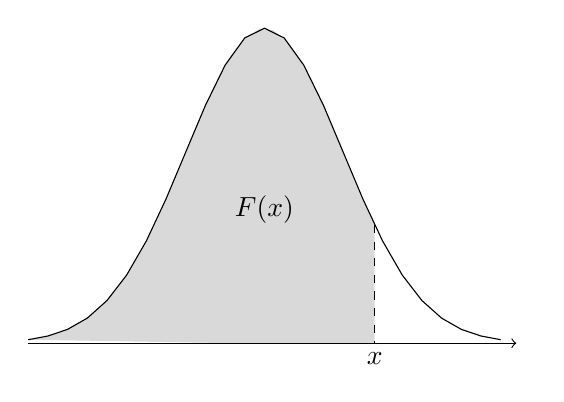
\begin{tikzpicture}
% define normal distribution function 'normaltwo'
    \def\normaltwo{\x,{4*1/exp(((\x-3)^2)/2)}}
 
% input y parameter
    \def\y{4.4}
 
% this line calculates f(y)
    \def\fy{4*1/exp(((\y-3)^2)/2)}
 
% Shade orange area underneath curve.
    \fill [fill=gray!30] (2.6,0) -- plot[domain=0:4.4] (\normaltwo) -- ({\y},0) -- cycle;
 
% Draw and label normal distribution function
    \draw[domain=0:6] plot (\normaltwo) node[right] {};
 
% Add dashed line dropping down from normal.
    \draw[dashed] ({\y},{\fy}) -- ({\y},0) node[below] {$x$};
 
% Optional: Add axis labels
%    \draw (-.2,2.5) node[left] {$f_Y(u)$};
    \draw (3,2) node[below] {$F(x)$};
 
% Optional: Add axes
    \draw[->] (0,0) -- (6.2,0) node[right] {};
%    \draw[->] (0,0) -- (0,5) node[above] {};
 
\end{tikzpicture}
%    \rule{6cm}{6cm} %to simulate an actual figure
\par\vspace{0pt}
  \end{minipage}%
  \begin{minipage}[b]{0.60\linewidth}
    \centering
\begin{tabular}{rr|rr|rr|rr}
  \hline
$x$ & $F(x)$ & $x$ & $F(x)$ & $x$ & $F(x)$ & $x$ & $F(x)$ \\ 
  \hline
0.050 & 0.520 & 0.750 & 0.773 & 1.450 & 0.926 & 2.150 & 0.984 \\ 
  0.100 & 0.540 & 0.800 & 0.788 & 1.500 & 0.933 & 2.200 & 0.986 \\ 
  0.150 & 0.560 & 0.850 & 0.802 & 1.550 & 0.939 & 2.250 & 0.988 \\ 
  0.200 & 0.579 & 0.900 & 0.816 & 1.600 & 0.945 & 2.300 & 0.989 \\ 
  0.250 & 0.599 & 0.950 & 0.829 & 1.650 & 0.951 & 2.350 & 0.991 \\ 
  0.300 & 0.618 & 1.000 & 0.841 & 1.700 & 0.955 & 2.400 & 0.992 \\ 
  0.350 & 0.637 & 1.050 & 0.853 & 1.750 & 0.960 & 2.450 & 0.993 \\ 
  0.400 & 0.655 & 1.100 & 0.864 & 1.800 & 0.964 & 2.500 & 0.994 \\ 
  0.450 & 0.674 & 1.150 & 0.875 & 1.850 & 0.968 & 2.550 & 0.995 \\ 
  0.500 & 0.691 & 1.200 & 0.885 & 1.900 & 0.971 & 2.600 & 0.995 \\ 
  0.550 & 0.709 & 1.250 & 0.894 & 1.950 & 0.974 & 2.650 & 0.996 \\ 
  0.600 & 0.726 & 1.300 & 0.903 & 2.000 & 0.977 & 2.700 & 0.997 \\ 
  0.650 & 0.742 & 1.350 & 0.911 & 2.050 & 0.980 & 2.750 & 0.997 \\ 
  0.700 & 0.758 & 1.400 & 0.919 & 2.100 & 0.982 & 2.800 & 0.997 \\ 
   \hline
\end{tabular}
\par\vspace{0pt}
\end{minipage}
\label{fig:test}
\end{figure}

\subsection{Вариант В}
\begin{questions}

\question Функция $f$ задана формулой 
\[
f(x)=\begin{cases}
x^2\sin(1/x), \; \text{ если } x\neq 0 \\
0, \; \text{ если } x = 0
\end{cases}
\]
\begin{parts}
\part[8]
Найдите правую, $f'_+(0)$, и левую, $f'_-(0)$, производные функции $f$ в точке $x=0$
\begin{solution}
Правая:
\[
\lim_{x\to 0^+}\frac{f(x)-f(0)}{x}=\lim_{x\to 0^+}\frac{x^2\sin(1/x)-0}{x}=\lim_{t\to +\infty} \frac{\sin t -0 }{t}=0
\]
Левая:
\[
\lim_{x\to 0^-}\frac{f(x)-f(0)}{x}=\lim_{x\to 0^-}\frac{x^2\sin(1/x)-0}{x}=\lim_{t\to -\infty} \frac{\sin t -0 }{t}=0
\]
\end{solution}

\part[2]
Существует ли производная функции $f$ в точке $x=0$?
\begin{solution}
Левая производная  равняется правой производной --- производная в точке $x=0$  равна $0$.
\end{solution}

\end{parts}

\question[10] Вычислите интеграл
\[
\int \sin( \ln x) \, dx
\]

\begin{solution}
Интегрируем два раза по частям:
\[
\int \sin( \ln x) \, dx = 	x \sin( \ln x)  - \int \cos( \ln x) \, dx = x \sin( \ln x)  -  x \cos( \ln x)  - \int \sin( \ln x) \, dx 
\]


Выражаем искомый интеграл:
\[
\int \sin( \ln x) \, dx =\frac{1}{2}\left(  x \sin( \ln x)  -  x \cos( \ln x)  \right)
\]
\end{solution}


\question Рассмотрим систему уравнений $Ax=b$, где 

\[
x=\begin{pmatrix}
x_1 \\
x_2 \\
x_3 
\end{pmatrix}, \; 
A=\begin{pmatrix}
1 & -2 & 0 \\
2 & 1 &  -1\\
-1 & 7 & \alpha  
\end{pmatrix}, \;
b=\begin{pmatrix}
1 \\
\beta \\
2
\end{pmatrix}.
\]

\begin{parts}
\part[6]
Найдите ранг и определитель матрицы $A$  как функции от параметра $\alpha$
\begin{solution}
Находим определитель (например, разложением по столбцу содержащему $\alpha$):
\[
\det A=5\alpha+5
\]
Определитель обращается в ноль только при $\alpha = -1$. Отсюда делаем вывод и про ранг матрицы.
При $\alpha = -1$ ранг матрицы равен двум, а при $\alpha \neq -1$ он равен трём.
\end{solution}
\part[4]
Определите количество решений системы в зависимости от значений параметров $\alpha$ и $\beta$
\begin{solution}
Если $\alpha \neq -1$, то решение системы единственно вне зависимости от $\beta$. При $\alpha=-1$ строки матрицы $A$ линейно зависимы. Матрица $A$ необратима и система либо не имеет решений, либо имеет бесконечное множество решений. Выясним зависимость между строками матрицы $A$, выразим третью строку матрицы через первые две:
\[
(-1;7;-1)=y_1(1;-2;0)+y_2(2;1;-1)
\]
Решая эту систему находим, что $y_1=-3$, а $y_2=1$. Если это же соотношение выполняется для столбца $b$, то система имеет бесконечное количество решений, иначе --- ни одного.
\[
2=-3\cdot 1 + 1\cdot \beta
\]

Следовательно, при $\alpha=-1$ и $\beta=5$ система имеет бесконечное количество решений, а при $\alpha=-1$ и $\beta\neq 5$ --- ни одного.
\end{solution}

%\part 
%Какие значения принимает ранг матрицы $C$, состоящей из матрицы $A$ и приписанного справа вектора $b$, $C=[A \; b]$, в зависимости от параметров $\alpha$ и $\beta$?

\end{parts}



\question Вектор-строка $b$ состоит из последовательных чисел от 4 до 1, $b=(4,3,2,1)$. Матрица $B$ задана соотношением $B=b^Tb$. 

\begin{parts}
\part[5]
Найдите собственные числа матрицы $B$
\begin{solution}
Ранг матрицы равен количеству ненулевых собственных чисел. Ранг произведения матриц не превосходит ранга сомножителей, поэтому ранг матрицы $B$ равен одному. Матрица $B$ ненулевая, поэтому у неё три нулевых собственных числа и одно ненулевое. 

Заметим, что $B\cdot b^T=(b^Tb)b^T=b^T(bb^T)=b^T\cdot (16+9+4+1)=30b^T$. Следовательно, четвёртое собственное число --- 30.
\end{solution}

\part[3]
Для максимального собственного числа укажите хотя бы один собственный вектор
\begin{solution}
Попутно в прошлом пункте мы нашли, что у числа $30$ есть собственный вектор $b^T=(4,3,2,1)^T$.
\end{solution}
\part[2]
Является ли матрица $B$ положительно определённой? Положительно полуопределённой?
\begin{solution}
У матрицы $B$ нулевые и положительные собственные числа. Она является положительно полуопределённой, а положительно определённой не является.
\end{solution}
\end{parts}

\question Задано дифференциальное уравнение 
\[
x\frac{dy}{dx}-y=(x+y)\ln \left( \frac{x+y}{x}  \right)
\]
\begin{parts}
\part[8]
Решите дифференциальное уравнение
\begin{solution}
Уравнение однородно (сохраняет вид при одновременном умножении  $x$  и $y(x)$  на постоянный множитель), поэтому можно использовать замену  $y(x)=z(x)x$. 
 
Заметим, что в области определения уравнения $x\neq 0$, поэтому решения при такой замене не теряются.
\[
x(z'+z)-zx=(x+zx)\ln \frac{x+zx}{x}
\]
\[
z'=\frac{(1+z)\ln(1+z)}{x}
\]
 
Переменные разделяются
\[
\frac{dz}{(1+z)\ln(1+z)}=\frac{dx}{x}
\]

\[
\int \frac{dz}{(1+z)\ln(1+z)}=\int \frac{dx}{x}
\]

\[
\ln |\ln(1+z)|=\ln|x| + \ln C_0, \; C_0>0
\]
постоянную интегрирования, которая может иметь любой знак, удобно в данном случае записать как логарифм положительной постоянной
\[
|\ln(1+z)|=C_0|x|, \; C_0>0
\]
 
Снимая модуль в левой части получаем постоянную любого знака

\[
\ln(1+z)=C|x|
\]
 
или
 
 \[
1+z=e^{C|x|}
\]

При $x=0$  уравнение не имеет смысла,  и постоянные интегрирования при положительных и при отрицательных значениях $x$  можно выбирать независимо. Иначе говоря, найденное множество интегральных кривых можно перечислить выражением
 
  \[
1+z=e^{Cx}
\]
 
Возвращая подстановку, получаем решение
 
\[
y(x)=\left(e^{Cx}-1 \right)x
\]

\end{solution}

\part[2]
Дайте схематический рисунок интегральных кривых
\begin{solution}
\begin{tikzpicture}
  \draw[->] (-3,0) -- (3,0) node[right] {$x$};
  \draw[->] (0,-3) -- (0,3) node[above] {$y$};
  \draw[domain=-3:1.2,smooth,variable=\x,blue] plot ({\x},{(exp(\x)-1)*\x});
  \draw[domain=-1.2:3,smooth,variable=\x,red] plot ({\x},{(exp(-\x)-1)*\x});
\end{tikzpicture}
\end{solution}

\end{parts}

\question[10] 
Исследуйте на экстремумы функцию $F(x,y)=16x^3+2y^3-24xy-15$

\begin{solution}
Найдем точки, подозрительные на экстремум, решая следующую систему уравнений:
\[
\begin{cases}
\frac{\partial F}{\partial x}=48x^2-24y=0 \\
\frac{\partial F}{\partial y}=6y^2-24x=0 \\
\end{cases}
\]
Получим точки:  $(0;0)$, $(1;2)$.
Далее необходимо проверить выполнение условий второго порядка. Для этого найдем матрицу вторых производных исследуемой функции:
\[
\begin{pmatrix}
96x & -24 \\
-24 & 12y 
\end{pmatrix}.
\]



Проверим знакоопределенность этой матрицы в каждой из найденных подозрительных точек.


Для точки  $(0;0)$ имеем следующую матрицу:  
$\begin{pmatrix}
0 & -24 \\
-24 & 0
\end{pmatrix}$. 
Находим угловые миноры, $\Delta_1=0$, $\Delta_2=0-24^2<0$. Следовательно, точка $(0;0)$  не является точкой экстремума.


Для точки $(1;2)$  имеем следующую матрицу:
$\begin{pmatrix}
96 & -24 \\
-24 & 24
\end{pmatrix}.$  
Находим угловые миноры, $\Delta_1=96>0$, $\Delta_2=96\cdot 24 -24^2>0$.  Следовательно, точка $(1;2)$  является точкой минимума.

Значение функции в этой точке: $F(x,y)=-31$.
\end{solution}

\question Рассмотрим функцию $Q(x,y)=x-2y$, аргументы которой удовлетворяют условию $b+ax^2+y^2=0$.
Найдите при каких значениях параметров $a$ и $b$  функция $Q(x,y)$:

\begin{parts}
\part[4]
будет иметь ровно одну условную стационарную точку, определите, является ли данная точка экстремумом;
\part[4]
будет иметь более одной условной стационарной точки, определите, являются ли данные точки экстремумами;
\part[2]
не будет иметь стационарных точек.  
\end{parts}

Указание. Для нахождения условных стационарных точек используйте метод множителей Лагранжа. Дополнительных исследований проводить не требуется. 


\begin{solution}

\begin{enumerate}
\item Если $a=0,b\le 0$, то ограничению удовлетворяют все значения аргумента x при $y=\sqrt{-b} $. В этом случае остается найти экстремум функции $x-2\sqrt{-b} $, которого, очевидно не существует. В данном случае стационарных точек нет. 

\item  Если $a\ge 0,b>0$, то ограничению не удовлетворяет ни одна точка. В данном случае стационарных точек нет.

\item  Остается рассмотреть два случая $a>0$, $b<0$ и $a<0$, $b$-любое. В этом случае используем метод множителей Лагранжа. Функция Лагранжа имеет вид $L\left(x,y,\lambda \right)=x-2y+\lambda \left(b+ax^{2} +y^{2} \right)$. Безусловные стационарные точки функции Лагранжа совпадают с условными стационарными точками в постановке задачи. Стационарная точка определяется из условий 
\end{enumerate}

\[
\left\{\begin{array}{c} {\frac{\partial }{\partial x} L\left(x,y,\lambda \right)=1+2\lambda ax=0} \\ {\frac{\partial }{\partial y} L\left(x,y,\lambda \right)=-2+2\lambda y=0} \\ {\frac{\partial }{\partial \lambda } L\left(x,y,\lambda \right)=b+ax^{2} +y^{2} =0} \end{array}\right. 
\] 

Решение данной системы уравнений существует не всегда. 

С.1) При условии, что $a\ne -16$ решением являются точки

 $\left\{\begin{array}{c} {x_{k} =-\frac{1}{2\lambda a} } \\ {y_{k} =\frac{1}{\lambda } } \end{array}\right. ,\, \lambda =\pm \sqrt{-\frac{1+4a}{ab} } $. Далее решение при положительном значении $\lambda $ назовем $\left(x_{1} ,y_{1} \right)$, а при отрицательном $\lambda $ - $\left(x_{2} ,y_{2} \right)$. Определим их тип. Достаточным условием существования условного экстремума в условной стационарной точке является постоянство знака второго дифференциала функции Лагранжа при учете условия. Второй дифференциал имеет вид: $d^{2} L\left(x,y,\lambda \right)=\frac{\partial ^{2} }{\partial x^{2} } L\left(x,y,\lambda \right)dx^{2} +2\frac{\partial ^{2} }{\partial x\partial y} L\left(x,y,\lambda \right)dxdy+\frac{\partial ^{2} }{\partial y^{2} } L\left(x,y,\lambda \right)dy^{2} $ Из ограничения следует, что 
\[
dy=-\left({\frac{\partial }{\partial x} F\left(x,y\right) \mathord{\left/{\vphantom{\frac{\partial }{\partial x} F\left(x,y\right) \frac{\partial }{\partial y} F\left(x,y\right)}}\right.\kern-\nulldelimiterspace} \frac{\partial }{\partial y} F\left(x,y\right)} \right)dx
\]
Таким образом, тип стационарной точки определяется знаком выражения 
\[
\begin{array}{l} {A=\frac{\partial ^{2} }{\partial x^{2} } L\left(x_{k} ,y_{k} ,\lambda _{k} \right)+2\frac{\partial ^{2} }{\partial x\partial y} L\left(x_{k} ,y_{k} ,\lambda _{k} \right)\left({\frac{\partial }{\partial x} F\left(x_{k} ,y_{k} \right) \mathord{\left/{\vphantom{\frac{\partial }{\partial x} F\left(x_{k} ,y_{k} \right) \frac{\partial }{\partial y} F\left(x_{k} ,y_{k} \right)}}\right.\kern-\nulldelimiterspace} \frac{\partial }{\partial y} F\left(x_{k} ,y_{k} \right)} \right)+} \\ {+\frac{\partial ^{2} }{\partial y^{2} } L\left(x,y,\lambda \right)\left({\frac{\partial }{\partial x} F\left(x_{k} ,y_{k} \right) \mathord{\left/{\vphantom{\frac{\partial }{\partial x} F\left(x_{k} ,y_{k} \right) \frac{\partial }{\partial y} F\left(x_{k} ,y_{k} \right)}}\right.\kern-\nulldelimiterspace} \frac{\partial }{\partial y} F\left(x_{k} ,y_{k} \right)} \right)^{2} } \end{array}
\]

В случае $a>0,b<0$ или $a\in \left(-\frac{1}{4} ,0\right),b>0$ $A=2\lambda (\frac{1}{4} +a)$. Тогда $\left(x_{1} ,y_{1} \right)$ является точкой минимума, а $\left(x_{2} ,y_{2} \right)$ является точкой максимума.

В случае $a<-\frac{1}{4} ,b<0$ $A=2\lambda (\frac{1}{4} +a)$. Тогда $\left(x_{1} ,y_{1} \right)$ является точкой максимума, а $\left(x_{2} ,y_{2} \right)$ является точкой минимума.

В случае $a\in \left(-\frac{1}{4} ,0\right),b<0$ или $a<-16,b>0$ выражение под корнем оказывается отрицательным и стационарных точек нет.

С.2) Если $a=-\frac{1}{4} $, то $\lambda =0$ и в силу линейности функции $Q(x,y)$ стационарных точек нет. 



Таким образом:

\begin{enumerate}
\item  Единственной стационарной точки не существует.

\item  Две стационарные точки существуют в случае:


$a>0,b<0$ или $a\in \left(-16,0\right),b>0$. Тогда $\left(x_{1} ,y_{1} \right)$ является точкой минимума, а $\left(x_{2} ,y_{2} \right)$ является точкой максимума.

$a<-16,b<0$. Тогда $\left(x_{1} ,y_{1} \right)$ является точкой максимума, а $\left(x_{2} ,y_{2} \right)$ является точкой минимума.

\item Во всех остальных случаях стационарные точки отсутствуют.
\end{enumerate}



\end{solution}

\question В лотерее каждый десятый билет выигрывает, причём цена билета равна десяти рублям, а выигрыш составляет семьдесят рублей. Билетов очень-очень много, поэтому выигрыши по ним можно считать независимыми.
\begin{parts}
\part[5] Каковы математическое ожидание и дисперсия выигрыша при покупке восьми билетов? Имеется в~виду выигрыш с учётом затрат на~приобретение, так что он может быть отрицательным.

\begin{solution}
Имеем дело с восемью испытаниями по схеме Бернулли с вероятностью успеха $0.1$.  Пусть $X$ --- число успехов (выигрышей). Тогда $\E(X)=8\cdot 0.1=0.8$, $\Var(X)=8\cdot 0.1\cdot 0.9=0.72$. Сумма выигрыша с учётом стоимости билетов $Y=70X-80$ (здесь 80 --- стоимость восьми билетов). Получаем ответ:
\[
\E(Y)=70\E(X)-80=70\cdot 0.8-80=-24,
\]
\[
\Var(Y)=70^2 \Var(X)=3528.
\]

Разбалловка: 5 баллов за пункт (а), по одному баллу за $\E(X)$, $\E(Y)$, связь $Y$ и $X$, $\Var(X)$, $\Var(Y)$.
\end{solution}

\part[5]
Некто покупает лотерейные билеты до~третьего выигрыша. С~какой вероятностью ему придётся купить ровно двенадцать билетов?

\begin{solution}
На этот раз число испытаний не ограничено. Чтобы двенадцатый билет был третьим выигрышным, он должен сам быть выигрышным (вероятность этого - $0.1$), а одиннадцать предыдущих должны содержать ровно два выигрыша, вероятность чего равна $C_11^2\cdot 0.1^2\cdot 0.9^9$. Искомая вероятность: $C_11^2\cdot 0.1^2\cdot 0.9^9\cdot 0.1\approx 0.02$.

Разбалловка: 5 баллов за пункт (б), из них два за формулу Бернулли.
\end{solution}
\end{parts}

\question Случайные величины $X_i$ независимы, а их распределение известно с~точностью до~параметра $p$:

\begin{center}
\begin{tabular}{lccc} \toprule
Значения & -3 & 0 & 1 \\ 
Вероятности & $0.1$ & $0.9-p$ & $p$ \\ \bottomrule
\end{tabular}
\end{center}

\begin{parts}
\part[5]
Пусть $p=0.3$. С какой вероятностью среднее в выборке $X_1, \ldots, X_{480}$ превысит значение $0.05$?
\begin{solution}
Найдём математическое ожидание и дисперсию $X_i$:
\[
\E(X_i)=-3\cdot 0.1+1\cdot p=p-0.3
\]
\[
\E(X_i^2 )=(-3)^2\cdot 0.1+1^2\cdot p=0.9+p,
\]
\[
\Var(X_i)=0.9+p-(p-0.3)^2=0.81+1.6p-p^2
\]
При $p=0.3$ получаем $\E(X_i )=0$, $\Var(X_i )=1.2$.
Объём выборки велик, так что выборочное среднее будет иметь приблизительно нормальное распределение: $\bar{X}\sim \cN(0,1.2/480=0.0025)$. Рассчитываем нужную нам вероятность, нормировав выборочное среднее:
\[
\P(\bar{X}>0.05)=\P\left(\bar{X} /\sqrt{0.0025}>0.05/\sqrt{0.0025} \right)=\P(\bar{X} /0.05>1)=0.159.
\]
Разбалловка: 5 баллов за пункт (а), по одному баллу за математическое ожидание, дисперсию, применение теоремы о распределении выборочного среднего (центральной предельной теоремы), нормирование, нахождение вероятности по таблицам;
\end{solution}

\part[5]
Докажите состоятельность оценки $\hat{p}=0.3+\frac{1}{n} \sum_{i=1}^n X_i$  для параметра $p$, где $n$ --- объём выборки.

\begin{solution}
Для доказательства состоятельности оценки достаточно показать, что она несмещённая, а её дисперсия стремится к нулю. Проверяем несмещённость:
\[
\E(\hat{p})=0.3+\E(\bar{X})=0.3+(p-0.3)=p.
\]
Ищем дисперсию: 
\[
\Var(\hat{p})=\Var(\bar{X})=(0.81+1.6p-p^2)/n.
\]
Ясно, что $\lim_{n\to\infty} \Var(\hat{p})=0$, так что оценка состоятельная.

Можно и не искать дисперсию $X_i$. Достаточно знать, что она конечна, а это следует из того, что множество значений $X_i$ конечно.


Разбалловка: 5 баллов за пункт (б), из них два – за достаточное условие состоятельности.
\end{solution}

\end{parts}



\question
Исследователь решил выяснить, есть ли связь между  гендерной принадлежностью и доходами индивида. В его распоряжении есть данные о заработных платах (переменная $wage$ --- средняя почасовая заработная плата в долларах), опыте (переменная $exper$ --- годы опыта) и поле  (дамми-переменная $gender$ принимает значение 1 для женщин). По 300-м наблюдениям он оценил следующее уравнение регрессии (предпосылки классической линейной регрессионной модели выполнены):
\[
\ln(wage_i) = \alpha + \beta_1 exper_i + \beta_2 exper_i^2 + \beta_3 gender_i + \varepsilon_i
\]

Результаты оценки уравнения представлены в таблице:
\begin{center}
\begin{tabular}{ccc} \toprule
Переменная & Коэффициент & Стандартная ошибка\\ \midrule
$exper$ & 0.0400 & 0.0134 \\
$exper^2$ & -0.0008 & 0.0004 \\
$gender$ & -0.0534 & 0.0847 \\
константа & -0.4860 & 0.2136 \\ \bottomrule
\end{tabular}
\end{center}


\begin{parts}
%\part[1]
%Почему исследователь решил включить в модель две переменных для наличия детей? 
%\begin{solution}
%Исследователь предполагает, что наличие детей разного возраста может оказывать разное по силе и направлению влияние на заработную плату женщины.
%\end{solution}

\part[1]
Выпишите оценённое уравнение регрессии.
\begin{solution}
\[
\widehat{\ln(wage_i)} = -0.4860 + 0.0400exper_i -0.0008 exper_i^2 - 0.0534 gender_i  
\]
\end{solution}

%\part[2]
%Как будут интерпретироваться величина коэффициент $\beta_3$ при переменной $educ$? 
%\begin{solution}
%При росте образования на 1 год заработная плата растёт примерно на $10.8$\%.
%\end{solution}

\part[6]
На уровне значимости 5\%-ов проверьте гипотезу о значимости связи гендерной принадлежности  и заработной платы против альтернативной об отсутствии связи. Выпишите нулевую и альтернативную гипотезы, укажите используемые формулы, рассчитайте необходимую статистику, укажите точный и асимптотический вид её распределения и сделайте вывод на её основе.

\begin{solution}
$H_0$: $\beta_3=0$, $H_a$: $\beta_3\neq 0$. $Z_{obs}=\frac{\hbeta_3}{se(\hbeta_3)}=-0.0534/ 0.0847\approx -0.6305$, $Z_{cr}\approx 1.95$. Расчетное значение тестовой статистики по модулю меньше критического, что не дает оснований отвергнуть нулевую гипотезу о незначимости коэффициента при переменной $kid6$. На уровне значимости 5\%-ов нет оснований утверждать, что существует связь между образованием и заработной платой. Точное распределение статистики --- $t_{296}$, асимптотическое --- $N(0;1)$.
\end{solution}


%\part[3]
%Рассчитайте  90\%-ый доверительный интервал для разницы математических ожиданий логарифмов заработной платы для женщины без детей и женщины с тремя детьми в возрасте 7, 10 и 13 лет при прочих равных условиях.
%\part
%Найдите точечную оценку для разницы в заработной плате женщины с опытом работы 5 лет, проучившейся 15 лет, с двумя детьми в возрасте 3 и 10 лет и для женщины с опытом работы 5 лет, проучившейся 15 лет, без детей.

%\begin{solution}
%Разница математических ожиданий логарифмов заработной платы для женщины без детей и женщины с детьми в возрасте 7, 10 и 13 лет при прочих равных условиях будет определяться значением коэффициента при переменной $kid18$.  Для расчета доверительного интервала для указанного коэффициента используется следующая формула: $[\hbeta_5 - Z_{cr} se(\hbeta_5); \hbeta_5 + Z_{cr} se(\hbeta_5)]$. 

%В данном случае $Z_{cr}=1.65$. Тогда нижняя граница интервала $-0.0125-1.65\cdot 0.0268=-0.0567$, верхняя граница $=-0.0125+1.65\cdot 0.0268=0.0317$.
%\end{solution}

\part[3]
Перечислите модельные предпосылки, которые были использованы при решении задачи

\begin{solution}
Детерминистическая версия:
\begin{enumerate}
\item Линейность зависимости $y$ от объясняющих переменных. 
\[
\ln(wage_i) = \alpha + \beta_1 exper_i + \beta_2 exper_i^2 + \beta_3 gender_i + \varepsilon_i
\]
\item Нет линейной зависимости между регрессорами. Матрица $X$ имеет полный ранг.
\item Нет систематической ошибки, $\E(\varepsilon_i)=0$
\item Гомоскедастичность $\Var(\varepsilon_i)=\sigma^2$
\item Некоррелированность ошибок $\Cov(\varepsilon_i,\varepsilon_j)=0$
\item Нормальность ошибок, $\varepsilon_i \sim N(0;\sigma^2)$
\end{enumerate}

Стохастическая версия:

\begin{enumerate}
\item Линейность зависимости $y$ от объясняющих переменных. 
\[
\ln(wage_i) = \alpha + \beta_1 exper_i + \beta_2 exper_i^2 + \beta_3 gender_i + \varepsilon_i
\]
\item С вероятностью один нет линейной зависимости между регрессорами. Матрица $X$ имеет полный ранг с вероятностью один.
\item Эндогенность, $\E(\varepsilon_i | X)=0$
\item Условная гомоскадастичность $\Var(\varepsilon_i |X)=\sigma^2$
\item Условная некоррелированность ошибок $\Cov(\varepsilon_i,\varepsilon_j |X)=0$
\item Нормальность ошибок, $\varepsilon_i \sim N(0;\sigma^2)$
\end{enumerate}

\end{solution}

\end{parts}

\end{questions}


\begin{figure}[b]
\caption{Таблица значений функции распределения для стандартной нормальной величины.}
  \begin{minipage}[b]{0.35\linewidth}
    \centering
    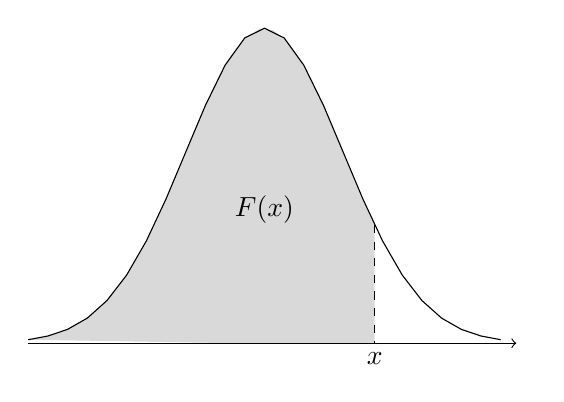
\begin{tikzpicture}
% define normal distribution function 'normaltwo'
    \def\normaltwo{\x,{4*1/exp(((\x-3)^2)/2)}}
 
% input y parameter
    \def\y{4.4}
 
% this line calculates f(y)
    \def\fy{4*1/exp(((\y-3)^2)/2)}
 
% Shade orange area underneath curve.
    \fill [fill=gray!30] (2.6,0) -- plot[domain=0:4.4] (\normaltwo) -- ({\y},0) -- cycle;
 
% Draw and label normal distribution function
    \draw[domain=0:6] plot (\normaltwo) node[right] {};
 
% Add dashed line dropping down from normal.
    \draw[dashed] ({\y},{\fy}) -- ({\y},0) node[below] {$x$};
 
% Optional: Add axis labels
%    \draw (-.2,2.5) node[left] {$f_Y(u)$};
    \draw (3,2) node[below] {$F(x)$};
 
% Optional: Add axes
    \draw[->] (0,0) -- (6.2,0) node[right] {};
%    \draw[->] (0,0) -- (0,5) node[above] {};
 
\end{tikzpicture}
%    \rule{6cm}{6cm} %to simulate an actual figure
\par\vspace{0pt}
  \end{minipage}%
  \begin{minipage}[b]{0.60\linewidth}
    \centering
\begin{tabular}{rr|rr|rr|rr}
  \hline
$x$ & $F(x)$ & $x$ & $F(x)$ & $x$ & $F(x)$ & $x$ & $F(x)$ \\ 
  \hline
0.050 & 0.520 & 0.750 & 0.773 & 1.450 & 0.926 & 2.150 & 0.984 \\ 
  0.100 & 0.540 & 0.800 & 0.788 & 1.500 & 0.933 & 2.200 & 0.986 \\ 
  0.150 & 0.560 & 0.850 & 0.802 & 1.550 & 0.939 & 2.250 & 0.988 \\ 
  0.200 & 0.579 & 0.900 & 0.816 & 1.600 & 0.945 & 2.300 & 0.989 \\ 
  0.250 & 0.599 & 0.950 & 0.829 & 1.650 & 0.951 & 2.350 & 0.991 \\ 
  0.300 & 0.618 & 1.000 & 0.841 & 1.700 & 0.955 & 2.400 & 0.992 \\ 
  0.350 & 0.637 & 1.050 & 0.853 & 1.750 & 0.960 & 2.450 & 0.993 \\ 
  0.400 & 0.655 & 1.100 & 0.864 & 1.800 & 0.964 & 2.500 & 0.994 \\ 
  0.450 & 0.674 & 1.150 & 0.875 & 1.850 & 0.968 & 2.550 & 0.995 \\ 
  0.500 & 0.691 & 1.200 & 0.885 & 1.900 & 0.971 & 2.600 & 0.995 \\ 
  0.550 & 0.709 & 1.250 & 0.894 & 1.950 & 0.974 & 2.650 & 0.996 \\ 
  0.600 & 0.726 & 1.300 & 0.903 & 2.000 & 0.977 & 2.700 & 0.997 \\ 
  0.650 & 0.742 & 1.350 & 0.911 & 2.050 & 0.980 & 2.750 & 0.997 \\ 
  0.700 & 0.758 & 1.400 & 0.919 & 2.100 & 0.982 & 2.800 & 0.997 \\ 
   \hline
\end{tabular}
\par\vspace{0pt}
\end{minipage}
\label{fig:test}
\end{figure}


\end{document}